% don't remove the folling lines, and edit the defintion of \main if needed
\documentclass[../report.tex]{subfiles}
\providecommand{\main}{..}
\IfEq{\jobname}{\currfilebase}{\AtEndDocument{\biblio}}{}
% until here
\begin{document}

\def\vub {\ensuremath{|V_{\uquark\bquark}|}\xspace}
\def\vcb {\ensuremath{|V_{\cquark\bquark}|}\xspace}
\def\qq {\ensuremath{q^{2}}\xspace}
\def\PMuNu{\decay{\Lb}{p \mun \neumb}}
\def\LcMuNu{\decay{\Lb}{\Lc \mun \neumb}}
\def\KMuNu{\decay{\Bs}{\Km \mup \neum}}
\def\DsMuNu{\decay{\Bs}{\Dsm \mup \neum}}
\def\Bq      {{\ensuremath{\B^0_\quark}}\xspace}
\def\Bqb     {{\ensuremath{\Bbar{}^0_\quark}}\xspace}
\def\dbtaunu {\decay{\B}{D^{(*)} \tau \nu}}
\def\dbmunu {\decay{\B}{D^{(*)} \mu \nu}}
\def\dbenu {\decay{\B}{D^{(*)} e \nu}}
\def\dmunu {\decay{\B}{D \mu \nu}}
\def\denu {\decay{\B}{D e \nu}}
\def\dsttaunu {\decay{\B}{D^{*} \tau \nu}}
\def\dstztaunu {\decay{\B}{D^{*0} \tau \nu}}
\def\dstptaunu {\decay{\B_{d}}{D^{*-} \tau^{+} \nu}}
\def\dstmunu {\decay{\B}{D^{*} \mu \nu}}
\def\dstenu {\decay{\B}{D^{*} e \nu}}
\def\dstpmunu {\decay{\B}{D^{*+} \mu \nu}}
\def\dstzmunu {\decay{\B}{D^{*0} \mu \nu}}
\def\dstlnu {\decay{\B}{D^{*} \ell \nu}}
\def\dblnu {\decay{\B}{D^{(*)} \ell \nu}}
\def\RDst {\ensuremath{\mathcal{R}(\Dstar)}\xspace}
\def\RDstp {\ensuremath{\mathcal{R}(\Dstarp)}\xspace}
\def\RD {\ensuremath{\mathcal{R}(D)}\xspace}
\def\RDb {\ensuremath{\mathcal{R}(D^{(*)})}\xspace}
\def\vub {\ensuremath{|V_{\uquark\bquark}|}\xspace}
\def\vcb {\ensuremath{|V_{\cquark\bquark}|}\xspace}
\def\qq {\ensuremath{q^{2}}\xspace}
\def\PMuNu{\decay{\Lb}{p \mun \neumb}}
\def\LcMuNu{\decay{\Lb}{\Lc \mun \neumb}}
\def\KMuNu{\decay{\Bs}{\Km \mup \neum}}
\def\DsMuNu{\decay{\Bs}{\Dsm \mup \neum}}
\def\vub {\ensuremath{|V_{ub}|}\xspace}
\def\vcb {\ensuremath{|V_{cb}|}\xspace}
\def\qq {\ensuremath{q^{2}}\xspace}
\def\PMuNu{\decay{\Lb}{p \mun \neumb}}
\def\LcMuNu{\decay{\Lb}{\Lc \mun \neumb}}
\def\KMuNu{\decay{\Bs}{\Km \mup \neum}}
\def\DsMuNu{\decay{\Bs}{\Dsm \mup \neum}}
\def        \DtoKspp        {\ensuremath{\D\to\KS\pip\pim}\xspace}
\def        \DtoKskk        {\ensuremath{\D\to\KS\Kp\Km}\xspace}
\def        \DtoKshh        {\ensuremath{\D\to\KS\hadron^+\hadron^-}\xspace}
\def        \BtoDpi         {\ensuremath{\Bpm\to\D\pipm}\xspace}
\def        \BtoDK          {\ensuremath{\Bpm\to\D\Kpm}\xspace}
\def        \BztoDstmuX     {\ensuremath{\Bz\to\Dstarpm\mu^\mp\nu_\mu X}\xspace}
\def        \hp            {\ensuremath{\hadron^+}\xspace}
\def        \hm            {\ensuremath{\hadron^-}\xspace}
\def        \BtoDKst       {\ensuremath{\Bz\to\PD\Kstarz}\xspace}
\def        \mpsq          {\ensuremath{m_{+}^{2}}\xspace}
\def        \mmsq          {\ensuremath{m_{-}^{2}}\xspace}
\def        \mpmsq          {\ensuremath{m_{\pm}^{2}}\xspace}
\def        \mmpsq          {\ensuremath{m_{\mp}^{2}}\xspace}
\def        \rb            {\ensuremath{r_B}\xspace}
\def        \db            {\ensuremath{\delta_B}\xspace}
\def        \g             {\ensuremath{\gamma}\xspace}
\def        \dpos          {\ensuremath{(\mpmsq,\mmpsq)\xspace}}
\def        \dbpos         {\ensuremath{(\mmpsq,\mpmsq)\xspace}}
\newcommand{\rbk}{\ensuremath{r_{B}^{DK}}\xspace}

\section{Testing the CKM unitarity}\label{sec:metro-CKM}
{\bf Author(s): Luca Silvestrini, J\'er\^ome Charles, Marco Ciuchini, Vincenzo Vagnoni, S\'ebastien Descotes-Genon, Olivier Deschamps}\\
(25 pages, TH:EXP= 50\%:50\%)

\subsection{Structure of the CKM matrix}

%\subsubsection{The CKM parameters}
% S. Descotes-Genon

In the Standard Model (SM), the weak charged-current transitions mix quarks of different generations, which is encoded in the
unitary Cabibbo-Kobayashi-Maskawa (CKM) matrix~\cite{Cabibbo:1963yz,Kobayashi:1973fv}. The relevant part of the SM 
 Lagrangian is
\begin{equation}\label{eq:chargeInteraction}
\mathcal{L}_{W^{\pm}} = -
\frac{g}{\sqrt{2}}\overline{U}_{i}\gamma^{\mu}\frac{1-\gamma^5}{2}\left(V_{\rm
CKM} \right )_{ij} D_{j} W_{\mu}^{+} + \mathrm{h.c.},
\end{equation}
where $g$ is the electroweak coupling constant, and $V_{\rm
CKM}=V_{u{L}}^\dag V_{d{L}}$ the unitary CKM matrix,
\begin{equation}\label{eq:ckmMatrix}
V_{\rm CKM} = \left(
\begin{array}{lcr}
V_{ud} & V_{us} & V_{ub} \\
V_{cd} & V_{cs} & V_{cb} \\
V_{td} & V_{ts} & V_{tb}
\end{array}
\right).
\end{equation}
The CKM matrix induces flavour-changing transitions inside and between generations in the charged currents at tree level ($W^\pm$ interaction). By contrast, there are no flavour-changing transitions in the neutral currents at tree level.

Experimentally, a strong hierarchy is observed  among the CKM matrix elements: transitions within the same generation are characterised by $V_{\rm CKM}$ elements of $\mathcal{O}(1)$, whereas
there is a suppression of $\mathcal{O}(10^{-1})$
between 1st and 2nd generations, $\mathcal{O}(10^{-2})$ between 2nd and 3rd and $\mathcal{O}(10^{-3})$ between 1st and 3rd.
This hierarchy is expressed by defining the four phase convention--independent
quantities,
\begin{equation}
\label{eq:lambda:A:rhoeta}
\lambda^2 =\frac{|V_{us}|^2}{|V_{ud}|^2+|V_{us}|^2}\,, \qquad
A^2\lambda^4=\frac{|V_{cb}|^2}{|V_{ud}|^2+|V_{us}|^2}\,, \qquad
\bar\rho+i\bar\eta=-\frac{V_{ud}V_{ub}^*}{V_{cd}V^*_{cb}}\,.
\end{equation}

The CKM matrix can be expanded in powers of the small parameter
$\lambda$ (which corresponds to the Cabibbo parameter $\sin{\theta_{C}}\simeq
0.22$)~\cite{Wolfenstein:1983yz} by exploiting the unitarity of
$V_\text{CKM}$. This
expansion yields the following parametrisation, valid up to
$\mathcal{O}\big(\lambda^{6}\big)$,
\begin{equation}\label{eq:ckmWolfenstein4}
V_{\rm CKM} = \left(
\begin{array}{ccc}
1-\frac{1}{2}\lambda^{2}-\frac{1}{8}\lambda^{4} & \lambda & A\lambda^{3}\left(\bar\rho -i\bar\eta\right) \\
-\lambda +\frac{1}{2}A^{2}\lambda^{5}\left[1-2(\bar\rho +i\bar\eta)\right] & 1-\frac{1}{2}\lambda^{2}-\frac{1}{8}\lambda^{4}(1+4A^{2}) & A\lambda^{2} \\
A\lambda^{3}\left[1-(\bar\rho +i\bar\eta)\right]~ &
~-A\lambda^{2}+\frac{1}{2}A\lambda^{4}\left[1-2(\bar\rho
+i\bar\eta)\right]~ & ~1-\frac{1}{2}A^{2}\lambda^{4}
\end{array}
\right).
\end{equation}
The CKM matrix is complex if $\bar\eta\ne 0$.  Furthermore, \CP is violated,  if
and only if $\bar\eta$ differs from zero. 
%To lowest order, the Jarlskog parameter measuring \CP violation in a convention-independent manner~\cite{Jarlskog:1985ht},
%\begin{equation}\label{eq:jarlskogValueWolf}
%J_{C\!P} \equiv \left|\Im\left(V_{i\alpha} V_{j\beta}
%V_{i\beta}^{*}V_{j\alpha}^{*}\right)\right| =
%\lambda^{6}A^{2}\bar\eta, \qquad \left( i\neq j,
%\alpha\neq\beta\right),
%\end{equation}
%is directly related to the \CP-violating parameter $\bar\eta$.

Orthogonality relations can be written involving two columns or two rows of the unitary CKM matrix, and they can be represented as triangles in the complex plane. It is standard to focus on the following orthogonality relation,
\begin{equation}
\label{eq:orthog:rel}
{V_{ud}V_{ub}^{*}}+{V_{cd}V_{cb}^{*}}+{V_{td}V_{tb}^{*}} = 0,
\end{equation}
as the three products of CKM elements 
%are involved in $B$-meson weak decays 
are of similar size, $O(\lambda^3)$. Fig.~\ref{fig:UTtriangle} shows the standard unitarity triangle (UT), obtained from \eqref{eq:orthog:rel} by rescaling with $V_{cd}V_{cb}^{*}$ the three terms in the orthogonality relation. 
%with apices located at $(0,0)$, $(1,0)$ and $(\bar\rho,\bar\eta)$. 
The apex of the UT is at $(\bar\rho,\bar\eta)$, while 
the angles 
%of the
%UT 
are related to the CKM matrix elements as
\begin{equation}
\alpha= \arg{\left(-\frac{V_{td}V_{tb}^{*}}{V_{ud}V_{ub}^{*}}\right)}, \qquad
\beta=\arg{\left(-\frac{V_{cd}V_{cb}^{*}}{V_{td}V_{tb}^{*}}\right)}, \qquad
\gamma\equiv\arg{\left(-\frac{V_{ud}V_{ub}^{*}}{V_{cd}V_{cb}^{*}}\right)}.
\end{equation}

\begin{figure}[!tb]
\centering
\includegraphics[width=0.6\linewidth]{section2/figures/ckmTriangle.pdf} 
\caption{
The standard CKM unitarity triangle. The parameters $\rho$ and $\eta$ are defined as 
$\rho+i\eta=\big(\bar\rho+i\bar\eta\big)\big(1-\lambda^2/2+O(\lambda^4)\big)$, with $\bar \rho, \bar \eta$ defined in \eqref{eq:lambda:A:rhoeta}.
}
\label{fig:UTtriangle}
\end{figure} 

    
\subsection{Current status of the constraints}

\td{1/2 page for each constraint}

\subsubsection{$|V_{ud}|,|V_{us}|,|V_{cd}|,|V_{cs}|$}
% S. Descotes-Genon

Accurate constraints on the first and second rows and columns of the CKM matrix come from leptonic decays, $\pi\to e\nu$, $K\to e\nu$, $K\to\mu\nu$, $\tau\to \pi\nu_\tau$,  $\tau\to K\nu_\tau$, $D\to \mu\nu$, $D_s\to \mu\nu$, and from semileptonic decays, $K\to\pi e\nu$, $D\to \pi e\nu$, $D_s\to Ke\nu$. The extraction of CKM matrix elements requires knowledge of hadronic inputs (decay constants for the leptonic decays, normalisations of the form factors at $q^2=0$ for the semileptonic decays) and electromagnetic/isospin corrections when available (i.e., for kaon and pion decays)~\cite{Antonelli:2010yf}. Another prominent input for $|V_{ud}|$ determination comes from the consideration of the superallowed $\beta$ decays of 20 different nuclei~\cite{Hardy:2014qxa,Towner:2015woa,Hardy:2018zsb}, which provides a very accurate constraint on $|V_{ud}|$. There are also other constraints, but less powerful due to experimental uncertainties and/or theoretical systematics that are difficult to assess.


\subsubsection{$|V_{cb}|$ and $|V_{ub}|$} 
% M. Ciuchini and L. Silvestrini

Tree-level semileptonic decays of beauty mesons and baryons allow for the extraction of $|V_{cb}|$ and $|V_{ub}|$. The current determination is dominated by the $B$-factories data on $B$ decays and by the measurement of $|V_{ub}|/|V_{cb}|$ from baryonic decays at LHCb. For $B$ decays, both inclusive and exclusive semileptonic decays have been used to extract $|V_{cb}|$ and $|V_{ub}|$. The two approaches have different sources of theoretical uncertainties: inclusive analyses rely on quark-hadron duality, on the heavy quark expansion and, for $|V_{ub}|$, on additional modeling; exclusive analyses require the knowledge of the relevant form factors over the entire kinematic range, a very difficult task for lattice QCD. Currently, the HFLAV averages for inclusive and exclusive determinations of $|V_{cb}|$ and $|V_{ub}|$ disagree at the $3\sigma$ level.
While recently the choice of the parameterization of the form factor dependence on the recoil for $B \to D^*$ decays has been shown to have a large impact on the extracted value of $|V_{cb}|$ \cite{Abdesselam:2018nnh,Bigi:2017njr,Grinstein:2017nlq}, the situation is still rather unclear. 

One way to deal with this is to assume that the uncertainty of each determination of $|V_{cb}|$ and $|V_{ub}|$ might have been underestimated, and perform a "skeptic combination" of all available data following the method of ref.~\cite{DAgostini:1999niu}, which is equivalent to the PDG prescription in one dimension, and is a straightforward generalization to the two-dimensional case of $|V_{cb}|$ and $|V_{ub}|$. The result 
%of this exercise
 is reported in Fig.~\ref{fig:UTfitvubvcb}, where in addition to the average we also plot the "indirect determination" obtained from all the other flavour observables.
 % in the SM. 
 The numerical results of the skeptic average are $|V_{cb}| = 0.0405 \pm 0.0011$, $|V_{ub}| = 0.00374 \pm 0.00023$, with correlation $\rho = 0.09$.

\begin{figure}[!tb]
\centering
\includegraphics[width=0.5\linewidth]{section2/figures/VubVcb_winter18.pdf} 
\caption{
Measurements of $|V_{cb}|$ and $|V_{ub}|$ from exclusive and inclusive $B$ decays (vertical and horizontal bands) and from \PMuNu and \LcMuNu (diagonal band), skeptical average and indirect determination of $|V_{cb}|$ and $|V_{ub}|$.
}
\label{fig:UTfitvubvcb}
\end{figure} 

It is reasonable to expect that progress on the lattice QCD determination of form factors in a larger kinematic range will allow Belle II to perform a much more parameterization-independent extraction of $V_{cb}$ from exclusive decays, hopefully reconciling it with the inclusive one. Also for $V_{ub}$, the much larger statistics should allow to get an insight on the origin of the discrepancy between inclusive and exclusive determinations, and provide a consistent determination of $V_{ub}$. 

\subsubsection{Angle $\alpha$}

% O. Deschamps
The constraints on the CKM angle $\alpha$ are derived from the isospin analysis of the charmless decay modes $B\to\pi\pi$, $B\to\rho\rho$ and $B\to\rho\pi$. This approach has the  interesting feature of being almost free from the hadronic uncertainties due to the QCD of binding quarks into the observed hadrons. Assuming the isospin symmetry and neglecting the electroweak penguin contributions, the amplitudes of the isospin SU(2)-conjugated modes are related, and  the measured branching fractions and asymmetries in the $\B^{\pm,0}\to(\pi\pi)^{\pm,0}$ and $B^{\pm,0}\to(\rho\rho)^{\pm,0}$ modes and the bilinear form factors in the Dalitz analysis of the neutral $B^{0}\to(\rho\pi)^0\to\pi^+\pi^-\pi^0$ decays provide enough observables to simultaneously extract the weak phase $\beta+\gamma=\pi-\alpha$ together with the hadronic tree and penguin contribution to each mode. The combination of the experimental data for the three decay modes above, mostly provided by the $B$-factories,  gives the world-average value at 68\% 
Confidence  Level (CL)\cite{Charles:2017evz}: 
%\begin{equation} \label{eq:alphadir}
$\alpha_{\rm dir} = (86.2^{+4.4}_{-4.0} \xspace\cup\xspace 178.4^{+3.9}_{-5.1})^\circ\,$.
%\end{equation}
The resolution is so far significantly larger than the theoretical uncertainty 
%related to hypotheses underlying the 
due to isospin SU(2) breaking, which
%analysis that 
may affect the  $\alpha_{\rm dir}$ determination at around $2^\circ$. The solution near $90^\circ$ is in  good agreement with the indirect determination obtained by the global fit of the flavour data\cite{CKMfitterwebsite}.
%\begin{equation}
%\alpha_{\rm ind}  = \val{92.5}{+1.5}{-1.1}{$^\circ$}\,.\label{eq:alphaInd}
%\end{equation}
% Considered separately, the $B\to\pi\pi$ and $B\to\rho\rho$ decays yield direct determinations of $\alpha$ in very good agreement with the indirect determination Eq.~(\ref{eq:alphaInd}), whereas the $B\to \rho\pi$ decay exhibits a 3$\sigma$ discrepancy. This discrepancy affects only marginally the combination Eq.~(\ref{eq:alphadir}), which is dominated by the results from $\rho\rho$ decays, and to a lesser extent $\pi\pi$ decays, whereas $\rho\pi$ modes play only a limited role.\\


A detailed analysis of the prospects for the CKM angle $\alpha$ has been performed in~\cite{Charles:2017evz}.
%, evaluating the individual impact of the charmless decay observables on the $\alpha$ determination. 
The global combination 
%of the  decay-specific determinations of 
$\alpha$ determinations is dominated by the $B\to\rho\rho$ data,
% that provides a constraint with a relative uncertainty at the level of 
constraining $\alpha$ with about 5\% uncertainty.  Improving the measurements of the neutral modes, especially the colour-suppressed $B^0\to\rho^0\rho^0$ decay, can have  sizeable impact. In $B\to\pi\pi$ system any sizable improvement is  driven by the increased accuracy in the measurement of the direct $\CP$ asymmetry in the colour-suppressed decay  $B^0\to\pi^0\pi^0$, potentially reachable through Dalitz decays $\pi^0\to\gamma e^+e^-$. However, all $\alpha$ measurements at subdegree precision must address isospin-breaking effects such as electroweak penguin contributions~\cite{Charles:2017evz,Gronau:2005pq}.

%\td{should this be moved to the experimental prospects?:}
%The experimental data is so far statistically limited for all the considered charmless modes. Due to the limited reconstruction efficiency of the neutral pions and the large associated background in the hadronic environment, the LHC contribution to the isospin analyses is so far confined to the final states reconstructed from charged pions only, i.e., the measurement of the branching ratio and the time-dependent $CP$-asymmetries in the  $B^0\to\pi^+\pi^-$ decay\cite{Aaij:2012as,Aaij:2018tfw}, and the branching ratio and fraction of longitudinal polarisation in the colour-suppressed decay mode, $B^0\to\rho^0\rho^0$ \cite{Aaij:2015ria}. A detailed analysis of the prospects for the CKM angle $\alpha$ has been performed in~\cite{Charles:2017evz}, evaluating the individual impact of the charmless decay observables on the $\alpha$ determination.

%The global combination of the  decay-specific determinations of $\alpha$ is dominated by the $B\to\rho\rho$ data,
%% that provides a constraint with a relative uncertainty at the level of 
%constraining $\alpha$ with about 5\% uncertainty.  Improving the accuracy of the $B^+\to\rho^+\rho^0$ branching ratio would  only marginally improve the determination of $\alpha$ (keeping all other observables unchanged). Improving the measurements of the neutral modes, especially the colour-suppressed $B^0\to\rho^0\rho^0$ decay, has larger impact,  driven by the $\CP$-asymmetries parameters.

%The subleading contribution to the combined $\alpha$ determination is provided by the $B\to\pi\pi$ system. Any sizable improvement on $\alpha_{\pi\pi}$ is  driven by the increased accuracy in the measurement of the direct $\CP$ asymmetry in the colour-suppressed decay  $B^0\to\pi^0\pi^0$. No time-dependent analysis has become available so far for the colour-suppressed mode due to the dominant di-photon decay of the neutral pions that  hinders the measurement of the decay time. However, the Dalitz decay $\pi^0\to\gamma e^+e^-$ (with low branching fraction) or the photon conversion in the detector material may allow one to measure the $B^0$ decay time in the future high-statistics flavour experiments.  In addition to a significant improvement on $\alpha$, the measurement of  $S^{00}_{\pi\pi}$ would  lift some of the discrete ambiguities and thus reduce the number of mirror solutions in the $B\to\pi\pi$ isospin analysis.

%The extraction of  $\alpha$ in the $B^0\to(\rho\pi)^0$ system relies on the analysis of the interference between the quasi two-body modes $B^0\to\rho^+\pi^-$, $B^0\to\rho^-\pi^+$ and  $B^0\to\rho^0\pi^0$. The Dalitz analysis of the three-pions final states permits a determination free from the discrete ambiguities usually affecting the (quasi) two-body modes, $B\to\rho\rho$ and $B\to\pi\pi$ . In addition, studies of the \decay{\Bp}{\pip\pip\pim} decay can provide useful constraints on the resonant structure of the decay, minimizing associated systematic uncertainties~\cite{Tandean:2002pe}.
%However, all $\alpha$ measurements at subdegree precision must address isospin-breaking effects such as electroweak penguin contributions~\cite{Charles:2017evz,Gronau:2005pq}.
%At LHCb, such analysis has to face the two fold difficulty of reconstructing the soft $\pi^0$ in the $\rho^+\pi^-$, $\rho^-\pi^+$ interference region and/or to separate the high-energy $\pi^0$ from the single photons from the radiative decays background in the  $\rho^0\pi^0$, $\rho^\pm\pi^\mp$ interference regions. At high luminosity, the analysis may take advantage of the Dalitz decays of the $\pi^0$ or the photon conversion in the detector material.

\subsubsection{Angle $\beta$} 
	The CKM angle $\beta$ is measured from the time-dependent CP asymmetry of $b\to c\bar c s$ decays, such as  
	%with a charmonium state and a $K$ meson in the final state. 
	%which measures Im$\lambda_f=$Im$(q/p \bar{A}_f/A_f)$. 
	%The archetypal $b\to c\bar c s$ process is 
	$B\to J/\psi K_S$.  The decay amplitude,  $A_{J/\psi K_S} = V_{cs}V_{cb}^* T + V_{us}V_{ub}^* P$, is dominated by the isoscalar tree-level amplitude $T$, while the subleading term $P$ is both loop and doubly Cabibbo suppressed. Neglecting $P$, 
	%the expression of 
	the time-dependent CP asymmetry, $a^{\CP}_t(B\to J/\psi K_S)=\sin2\beta\,\sin(\Delta m_B\, t)$,  has a single oscillatory term, the amplitude of which gives experimental access to $\sin2\beta$ (the fourfold ambiguity in $\beta$ can be reduced through time-dependent transversity analysis of $B\to J/\psi K^*$, sensitive to $\cos2\beta$).
	%, providing a determination of the CKM angle with a four-fold ambiguity.~\footnote{This ambiguity can be reduced using measurements sensitive to $\cos2\beta$ such as the time-dependent transversity analysis of $B\to J/\psi K^*$.} 
	The $P=0$ approximation is justified as long as the relative error on $\sin2\beta$ is larger than the correction induced by the subleading term $\sim \lambda^2 P/T$. The present relative uncertainty on $\sin2\beta$ from various charmonium states, including $J/\psi$ / $\psi(2S)$ / $\chi_{c1}$ / $\eta_c$ $K_S$, $J/\psi K_L$, $\psi(nS)K^0$, is about $2.4\%$. Double Cabibbo suppression amounts to $5\%$ and $P/T < 1$ is expected. Yet the precise suppression due to $P/T$ is unknown, likely ranging between some tens and a few percent, the latter estimate given by the perturbative evaluation of the penguing amplitude. Thus, depending on the actual value of $P/T$, the subleading amplitude could be a limiting factor for the extraction of $\sin2\beta$ already now or, in the opposite case, be safely neglected
	down to an experimental precision of few permille. In order to bound the subleading amplitude, one can use $SU(3)$ flavour (or U-spin) related decays where the penguin contribution is not suppressed, such as $B_s\to J/\psi K_s$ or $B\to J/\psi \pi$~\cite{Fleischer:1999nz,Ciuchini:2005mg,Faller:2008zc,Ciuchini:2011kd,Jung:2012mp,DeBruyn:2014oga}. Measuring branching ratios and (time-dependent) CP asymmetries, it is possible to extract the correction to $\sin2\beta$ induced by the subleading term and the corresponding uncertainty, due to the experimental errors and $SU(3)$-breaking effects. The latter, being proportional to a suppressed amplitude, are expected to be at the permille level.
	
	With present data, the typical shift in $\beta$ is $0.5$--$1^\circ$ with about $100\%$ uncertainty, dominated by the experimental uncertainties. Improvements in the measurement of the time-dependent asymmetry in $B\to J/\psi K_S$ should therefore be accompanied by a corresponding improvement in the measurement of the control channels in order to keep the subleading amplitude under control and extract $\sin2\beta$ with a subpercent precision.
	It is worth mentioning that a complemetary approach proposing a theoretical computation of the subleading amplitude using an OPE based on soft-collinear factorization in QCD can be found in Ref.~\cite{Frings:2015eva}.
	Assuming that the subleading amplitude is kept under control, the uncertainty on the indirect determination of $\sin2\beta$ from the UT analysis is expected to go from the present 4.5\% down to 0.6\%, providing an improved sensitivity to NP in the $B$--$\bar B$ mixing amplitude, as discussed further below.


\subsubsection{Angle $\gamma$}

% S. Descotes-Genon

The current best sensitivity is obtained from charged 
$B$ decays into $\tilde{D} K^-$, $\tilde{D}^{*} K^-$, and $\tilde{D} K^{*-}$, where $\tilde{D}$
is a $D^0$ or $\overline{D}^0$ meson decaying to the same final state. The $D^0$ is produced through
the leading $b \to c$ transition, with the amplitude ${\cal A}_{b\to c}\propto \lambda^3$, and $\overline{D}^0$ in the
% through 
CKM and colour-suppressed $b \to u$ transition,  ${\cal A}_{b\to u}\propto \lambda^3 \big({\bar{\eta}^2+\bar{\rho}^2}\big)^{1/2} e^{i( \delta_B - \gamma)}$.
%The amplitude ${\cal A}_{b\to c}$ is proportional 
%to $\lambda^3$, while the amplitude  ${\cal A}_{b\to u}$ is proportional
%to $\lambda^3 \sqrt{\bar{\eta}^2+\bar{\rho}^2}$ $\times e^{i( \delta_B - \gamma)}$.
Since $D^0$ and $\overline{D}^0$ decay to a common final state, 
the interference between the two tree amplitudes leads to observables that 
depend on the relative weak phase $\gamma$ and results in different 
$B^+$ and $B^-$ decay rates.
The size of this interference also depends on the magnitude of the ratio
of the two amplitudes, $r_B\equiv \vert {\cal A}_{b\to u}/$ ${\cal A}_{b\to c} \vert$,
and the relative strong phase $\delta_B$.
The value of $r_B$, which determines the size of the direct \CP\ asymmetry,
is predicted~\cite{Gronau:2002mu} to lie in the range 0.05--0.2. Experimental sensitivity to $\gamma$
decreases with smaller $r_B$.
%The smaller
%the $r_B$ is, the smaller is the experimental sensitivity to $\gamma$.

There are several different methods that exploit the above interference pattern: the Gronau-London-Wyler (GLW)
method~\cite{Gronau:1990ra,Gronau:1991dp} where the neutral $D$ meson is
reconstructed in a \CP\ eigenstate; the Atwood-Dunietz-Soni (ADS)
method~\cite{Atwood:1994zm,Atwood:1996ci,Atwood:2000ck} where the $D^0$ meson,
associated with the ${\cal A}_{b\to c}$ amplitude, is required to decay to a doubly
Cabibbo-suppressed decay (DCSD), while the $\overline{D}^0$ meson, associated with the
${\cal A}_{b\to u}$ amplitude, decays to a Cabibbo-favoured final state, such as
$K^+\pi^-$; the Giri-Grossman-Soffer-Zupan (GGSZ) method~\cite{Giri:2003ty} 
where the neutral $D$ meson is reconstructed in self-conjugate three-body 
final state such as $K_S^0 h^+ h^-$ (where $h=\pi$ or $K$). These $\gamma$ extraction techniques 
rely on clean theoretical assumptions since the decay amplitudes 
are completely tree-level dominated, to an excellent 
approximation~\cite{Brod:2013sga}.
All variants are sensitive to the same $B$ decay parameters and can therefore
be combined in a single fit to extract the common weak phase $\gamma$, as well 
as the hadronic parameters associated with each method.

\subsubsection{Angle $\beta_s$}
	The angle $\beta_s$ belongs to the squeezed UT $\sum_{q_u} V_{q_u b}^*V_{q_u s}=0$ instead of the usual $\sum_{q_u} V_{q_u b}^*V_{q_u d}=0$. Given its reduced sensitivity to $\bar{\rho}$ and $\bar{\eta}$, it is not a strong constraint in the UT plane. On the other hand, the UT analysis provides a very precise indirect determination of its value that can be compared with the direct determination extracted from time-dependent transversality analysis of $B_s\to\phi K_S$. At present, we have $\beta_s^\mathrm{direct} = 0.60\pm 0.88$ and  $\beta_s^\mathrm{UTA} = 1.06\pm 0.03$. The future uncertainties of the direct and indirect determinations are expected to be $\pm 0.01$ and $\pm 0.007$ respectively, allowing for a deeper investigation of BSM contributions to $B_s$--$\bar{B}_s$ mixing amplitude.
	It is worth noting that, similarly to the measurement of phase $\beta$, the shifts of a few degrees in the value of $\beta_s$ extracted from the time-dependent analysis caused by the subleading amplitude cannot be excluded. These shifts, however, now  produce a much larger relative uncertainty, since $\beta_s$ itself is doubly Cabibbo suppressed. %Indeed, for this reason, s
	Some control of doubly Cabibbo suppressed contributions is thus required to meaningfully extract $\beta_s$ at the SM level.
	This can be achieved by using 
	%Also here, this control can be provided by 
	the $SU(3)_f$ related channels, with the additional caveat that $\phi$ is an (almost equal) admixture of $SU(3)_f$ octet and singlet, introducing an additional source of symmetry breaking.


\subsubsection{$K-\bar{K}$ mixing} 
The CP-violating parameter $\varepsilon_K$, historically the first constraint in the UT plane, is becoming limited by long-distance contributions.
In the last years, the improvements in the constraining power of $\varepsilon_K$ have come from new determination of the bag parameter, $B_K$, on the lattice. Nowadays, the theoretical error on $B_K$  is approaching percent level. The dominating uncertainty in the SM prediction of $\epsilon_K$ comes from the long-distance contributions, the best estimate for which has an error of $2\%$~\cite{Buras:2010pza}, and no clear path of improvement. A breakthrough could come from developing ideas for computing these terms on the lattice, using recent techniques to cope with the non-local operators.


\subsubsection{$B_d-\bar{B}_d$ and $B_s-\bar{B}_s$ mixing}

% S. Descotes-Genon

The dispersive and absorptive contributions to  $B_d$ and $B_s$ mixing are described by $2\times2$ matrices, 
%can be described upon introducing
%the mass and decay matrices, 
$M^q=M^{q\dagger}$ and
$\Gamma^q=\Gamma^{q\dagger}$, respectively ($q=d,s$). 
They describe the quantum-mechanical evolution 
%matrices are involved in the evolution
%operator for the quantum-mechanical description 
of the  $B_q-\overline{B}_q$ system. 
%oscillations (with $q=d$ or $q=s$).
Their diagonalisation defines the physical eigenstates $\ket{B^q_H}$ and
$\ket{B^q_L}$ with masses
$M^q_H,\,M^q_L$ and decay rates $\Gamma^q_H,\,\Gamma^q_L$.
One can reexpress these quantities in terms of three parameters:   $|M_{12}^q|$,
$|\Gamma_{12}^q|$ and the relative phase $\phi_q=\arg(-M_{12}^q/\Gamma_{12}^q)$.
The SM prediction for the mass splitting, $\Delta m_q=M_H^q-M_L^q$,  is dominated by boxes involving top quarks, and is given by,
	\begin{equation}
	\label{eqof-dmd}
	   \dm_q = \frac{G_F^2}{6 \pi^2}\eta_B m_{B_q}f_{B_q}^2 {\hat{B}}_q
		  m_W^2 S(x_t) \left|V_{tq} V_{tb}^*\right|^2,
	\end{equation}
with  the Inami-Lim function $S(x_t)$~\cite{Inami:1980fz} evaluated at $x_{t}=\overline{m}_t^2/m_W^2$, while
$\eta_B$ encodes the perturbative QCD corrections, 
%. The value and uncertainty for the perturbative QCD
%correction $\eta_{B}$ was 
originally estimated in Ref.~\cite{Buchalla:1995vs}.
Using up-to-date $\alpha_{s}$ and the top-quark mass gives $\eta_{B} = 0.5510 \pm 0.0022$~\cite{Lenz:2010gu}.
%The prediction involves also non-perturbative inputs, t
The decay constant $f_{B_q}$ and the so-called bag parameter, $\hat{B}_q$, parametrize the nonperturbative hadronic matrix elements.  
%(which is defined by comparison with the vacuum insertion approximation).

The translation of the measured value for $\Delta m_d$ into constraints
on the CKM parameter combination ${|V_{td}^{\phantom{*}} V_{tb}^{*}|}^{2}$
is limited at present by uncertainties in the lattice QCD calculation of the
hadronic parameters $f_{B_{d}},  B_{B_{d}}$. The ratios $f_{B_s}/f_{B_d}$ and $B_{B_s}/B_{B_d}$ are much better determined, so that 
%it makes sense to consider 
$\Delta m_d/\Delta m_s$ gives a much better constraint in the $(\bar \rho,\bar \eta)$ plane, see Fig. \ref{CKMfitterSummer2018}. 
%The SM prediction for $\Delta m_s$ depends on CKM matrix elements $\vert V^*_{ts}V^{\phantom{*}}_{tb}\vert^2$, which only weakly depend on $\bar \rho,\bar \eta$.
%%   of the Standard Model prediction  on
%%$\bar \rho-\bar \eta$ coordinates appears to be very weak through the relevant
%%CKM matrix elements term $\vert V^*_{ts}V^{\phantom{*}}_{tb}\vert^2$.
%When combined with the $\Delta m_d$ measurement the measured $\Delta m_s$ value
%improves the ${|V_{td}^{\phantom{*}} V_{tb}^{*}|}^{2}$ constraint obtained from
%$\Delta m_d$. 
The hadronic
parameters, $f_{B_{s}}$, $B_{B_{s}}$, as well as $f_{B_s}/f_{B_d}$ and $B_{B_s}/B_{B_d}$,
are set to have their errors significantly reduced  by future lattice QCD computations, see Table \ref{table:Proj}.


\begin{table}
\caption{Constraints used for the global fit by CKMFitter collaboration, and the main experimental inputs involved (more information, especially for the theory inputs used, can be found in Ref.~\cite{CKMfitterwebsite}).
 \label{tab:expinputs}}
\begin{center}
\begin{tabular}{cccccc}
\hline\hline
CKM  &  Process  & \multicolumn{4}{c}{Observables}\\
\hline
$|V_{ud}|$ & $0^+\to 0^+$ $\beta$
                  & $|V_{ud}|_{\rm nucl}$&=& $0.97420\pm 0 \pm 0.00021$
                  &   \\
 %                   \hline
\multirow{4}{*}{\qquad$|V_{us}| \left\{\begin{matrix}&\\&\\&\\&\end{matrix}\right.$}  & $K\to\pi\ell\nu$ 
                  & $|V_{us}|_{\rm semi}f_+(0)$&=& $0.2165 \pm 0.0004$ & 
                  \\
                 &  $K\to e\nu_e$ 
                 & ${\cal B}(K\to e\nu_e)$&=&$ (1.582\pm 0.007)\cdot 10^{-5}$ & 
                 \\
                &  $K\to \mu\nu_\mu$ 
                &  ${\cal B}(K\to \mu\nu_\mu)$&=& $0.6356\pm 0.0011$
                & \\
                 &  $\tau \to K \nu_\tau$ 
                 & ${\cal B}(\tau \to K\nu_\tau)$&=&$0.006960\pm 0.000096$
                 & \\
 %                \hline
\multirow{2}{*}{$|V_{us}|/|V_{ud}|\left\{\begin{matrix}&\\&\\&\end{matrix}\right.$ }                &  $K(\pi)\to \mu\nu$ & 
                 $\displaystyle \frac{{\cal B}(K\to \mu\nu_\mu)}{{\cal B}(\pi \to \mu\nu_\mu)}$
                         &=&$(1.3367\pm 0.0029)\cdot 10^{-2}$
                 & 
                  \\
                 &  $\tau\to K(\pi)\nu$ &   
                 $\displaystyle \frac{{\cal B}(\tau \to K\nu_\tau)}{{\cal B}(\tau \to \pi\nu_\tau)}$
                        &=& $(6.438\pm 0.094)\cdot 10^{-2}$
                 &  \\
 %                \hline
$|V_{cd}|$ & $D\to \mu\nu $ & ${\cal B}(D\to \mu\nu)$ &=& $(3.74\pm 0.17)\cdot 10^{-4}$ 
                   & 
                   \\
 %                  \hline
\multirow{2}{*}{$\qquad|V_{cs}|\left\{\begin{matrix}&\\&\end{matrix}\right.$}   & $D_s\to \tau\nu$ 
                   & ${\cal B}(D_s\to \tau\nu)$&=& $(5.55\pm 0.24)\cdot 10^{-2}$ 
                   &  
                   \\
                   & $D_s\to \mu\nu$ 
                   & ${\cal B}(D_s\to \mu\nu_\mu)$&=& $(5.39\pm 0.16)\cdot 10^{-3}$ 
                   &  \\
 %                  \hline
\multirow{2}{*}{$\qquad|V_{ub}| \left\{\begin{matrix}&\\&\end{matrix}\right.$ }   & semilept. decays 
                  & $|V_{ub}|_{\rm semi}$ &=& $(3.98\pm 0.08\pm 0.22)\cdot 10^{-3}$ 
                  & \\
                  & $B\to \tau\nu$ 
                  & ${\cal B}(B\to\tau\nu)$ &=& $(1.08\pm 0.21)\cdot 10^{-4}$ & 
                  \\
 %                 \hline
$|V_{cb}|$ & semilept. decays
                 & $|V_{cb}|_{\rm semi}$ &=& $(41.8\pm 0.4 \pm 0.6)\cdot 10^{-3}$ & 
                 \\
$|V_{ub}/V_{cb}|$ & $\Lambda_b$ decays
      & 
      $\frac{{\cal B}(\Lambda_p\to p\mu^-\bar\nu_\mu)_{q^2>15}}{{\cal B}(\Lambda_p\to \Lambda_c\mu^-\bar\nu_\mu)_{q^2>7}}$ 
                &=& $(0.947\pm 0.081) \times 10^{-2}$ & \\
%\hline
$\alpha$ & $B\to\pi\pi$, $\rho\pi$, $\rho\rho$ 
                & \multicolumn{3}{c}{branching ratios, CP asymmetries} & 
                \\
 %               \hline
$\beta$   & $B\to (c\bar{c}) K$ 
               & $\sin(2\beta)_{[c\bar{c}]}$ &=& $0.699\pm 0.017$ 
               & \\
%\hline
$\gamma$ & $B\to D^{(*)} K^{(*)}$ 
                 & \multicolumn{3}{c}{GGSZ, GLW, ADS methods}
                 &   \\
 %\hline
\multirow{2}{*}{$\quad V_{tq}^*V_{tq'} \left\{\begin{matrix}&\\&\end{matrix}\right.$ }        & $\Delta m_d$ 
                & $\Delta m_d$ &=& $0.5065\pm 0.0019$ ps${}^{-1}$
                & 
                \\
                 & $\Delta m_s$ & $\Delta m_s$ &=& $17.757\pm 0.021$ ps${}^{-1}$ 
                 & 
                 \\
 %                \hline
$V_{tq}^*V_{tq'},V_{cq}^*V_{cq'}$  
      & $\epsilon_K$ & $|\epsilon_K|$ &=& $(2.228\pm 0.011)\cdot 10^{-3}$
       & \\
       \hline\hline
\end{tabular}
\end{center}
\end{table}

\subsection{Combined contraints on the CKM parameters}\label{sec:2018ckmfit}
Due to its economical structure in terms of only four parameters 
%and
%its consequences for \CP violation, 
the CKM matrix can be
determined through many different quark transitions, both the 
 $\Delta F = 1$ decays and the $\Delta F=2$ neutral-meson mixing transitions. A consistent determination of the four CKM parameters from all these processes is a fundamental test of the Kobayashi-Maskawa mechanism. 
Extracting from data the information on the four CKM parameters poses both experimental and theoretical challenges.
% for both experimentalists and theorists. 
First of all, the SM depends on a number of other parameters, masses and couplings, which are not predicted within the SM, but rather need to also be determined experimentally. An additional difficulty relates to the presence of strong interactions, binding quarks into hadrons. This is responsible for most of the theoretical uncertainties in the determinations of CKM matrix elements. 


\subsubsection{Statistical approaches}



The CKMfitter group determines the CKM parameters from a large set of flavour physics constraints using a standard $\chi^2$-like frequentist approach, in addition to a specific (Rfit) scheme to treat theoretical uncertainties~\cite{Charles:2004jd,Charles:2011va,Charles:2015gya}. The set of experimental observables, denoted $\vec {\cal O}_{exp}$, is measured in terms of likelihoods that can be used to build a \chisq-like test statistic,
\begin{equation}
\chi^2(\vec{p})=-2\log {\mathcal{L}}(\vec {\cal O}_{exp}-\vec {\cal O}_{th}(\vec p)),
\end{equation}
where $\vec {\cal O}_{th}(\vec p)$ represent the theoretical value of the observables for the N fixed parameters $\vec p$. The absolute minimum value of the test statistic, $\chi^2_{\rm min}$, quantifies the agreement of the data with the theoretical model, once converted into a $p$-value (interpreting $\chi^2(\vec{p})$
as a random variable distributed according to a $\chi^2$ law, generally relying on Wilks' theorem). It is also possible to perform the metrology of specific parameters of the model~\cite{Hocker:2001xe,Charles:2004jd,Charles:2016qtt}. Indeed, if we consider the $\vec\mu$ hadronic parameters as ``nuisance parameters'', 
we can define the test statistic from the \chisq difference:
\begin{equation}\label{eq:deltachisq}
 \Delta\chi^2(\alpha) = \min_{\vec\mu}[\chi^2(\alpha)] - \chi^2_{\rm min}
\end{equation}
where  $\min_{\vec\mu}[\chi^2(\alpha)]$ is the value of  \chisq, minimised with respect to the nuisance parameters for a  fixed $\alpha$ value. This test statistic assesses how a given hypothesis on the true value of $\alpha$ agrees with the data, irrespective of the value of the nuisance parameters. Confidence intervals on $\alpha$ can be derived from the resulting $p$-value, which is computed assuming that $\Delta\chi^2(\alpha)$ is \chisq-distributed with one degree of freedom:
\begin{equation}\label{eq:prob}
 p(\alpha) = {\rm Prob}(\Delta\chi^2(\alpha),N_{dof}=1)\,, \qquad  {\rm Prob}\!\left(\Delta \chi^2,N_{dof}\right)=\frac{\Gamma(N_{dof}/2,\Delta\chi^2/2)}{\Gamma(N_{dof}/2)}\,.
\end{equation}
Confidence intervals at a given confidence level (CL) are obtained by selecting the values of $\alpha$ with a $p$-value larger than $1-$CL.

In addition to the frequentist statistical treatment outline above, the CKMfitter collaboration relies on a specific treatment of theoretical uncertainties (i.e., systematics not scaling with the size of the sample) which are particularly relevant in the field of flavour physics (e.g. uncertainties on hadronic matrix elements). The current approach is the so-called Rfit~\cite{Hocker:2001xe,Charles:2004jd,Charles:2016qtt} model, corresponding to a constraint to $\chi^2$ restricting the value of the theoretical parameter/observable to a range, without any possibility to exceed this range. Most of the systematic uncertainties come from lattice QCD. The CKMfitter collaboration follows the recommendations of the Flavour Lattice Averaging Group~\cite{Aoki:2016frl} and uses a specific procedure to perform the average of the lattice inputs based on the Rfit model combined with a linear addition of systematic uncertainties for the individual inputs~\cite{Charles:2016qtt}.

	The UTfit collaboration follows a Bayesian approach to combine the constraints in the UT plane.  Bayesian statistics allows for a unified treatment of systematic and theoretical uncertainties in a scheme of "updating of knowledge" from prior to posterior distributions that is quite intuitive and easy to implement.
Following Bayes theorem, the (unnormalized) posterior p.d.f.\ for $\bar\rho$ and $\bar\eta$ (given the constraints) is written as
	\begin{equation}
	f(\bar\rho,\bar\eta|\mathbf{\hat{c}}, \mathbf{\hat{f}}) \propto 
	{\cal L}(\mathbf{\hat{c}}\,|\,\bar\rho,\bar\eta,\mathbf{f})\, f_0(\bar\rho,\bar\eta)\,,
	\label{eq:flat_inf}
	\end{equation}
	where $\mathbf{\hat{c}}=\{c_1,c_2,\dots,c_M\}$ is a set of measured constraints, whose theoretical expressions are given by the functions $c_j(\bar\rho,\bar\eta;\mathbf{x})$ depending on $\bar\rho$, $\bar\eta$, and a set of additional experimental and theoretical parameters ${\mathbf x}=\{x_1,x_2,\dots,x_N\}$, $f_0(\bar\rho,\bar\eta)$ is the prior p.d.f.\ for $\bar\rho$ and $\bar\eta$, assumed to be flat on the UT plane, and the effective overall likelihood ${\cal L}(\mathbf{\hat{c}}\,|\,\bar\rho,\bar\eta,\mathbf{f})$ is
    \begin{equation}
    {\cal L}(\mathbf{\hat{c}}\,|\,\bar\rho,\bar\eta,\mathbf{f})
    = \int 
    \prod_{j=1,{\rm M}}f_j(\hat{c}_j\,|\,\bar\rho,\bar\eta,\mathbf{x})
    \prod_{i=1,{\rm N}}f_i(x_i)\, \mbox{d}{ x_i}\,.
    \label{eq:lik_int}
    \end{equation}
	The p.d.f.\ $f_i=\{f_1,f_2,\dots,f_N\}$ are the prior distributions of the parameters, while  $f_j(\hat{c}_j\,|\,\bar\rho,\bar\eta,\mathbf{x})$ are the conditional probabilities of $\hat{c}_j$ given $\bar\rho$, $\bar\eta$, and $\mathbf{x}$, that in the Gaussian approximation become
    \begin{equation}	
	f_j(\hat{c}_j\,|\,\bar\rho,\bar\eta,\mathbf{x})=\frac{1}{\sqrt{2 \pi}\,\sigma(c_j)}
	\exp\left[-\frac{(c_j(\bar\rho, \bar\eta; \mathbf{x})-
		\hat{c}_j)^2}{2\,\sigma^2(c_j)}\right]\,.
    \end{equation}
    The integration in eq.(\ref{eq:lik_int}) is usually carried out using Monte Carlo methods. More details on the Bayesian approach of the UTfit collaboration can be found in ref.\cite{Ciuchini:2000de}.


% S. Descotes-Genon
\subsubsection{Current combined constraints on the CKM parameters}
In the CKMfitter case,
Table~\ref{CKMfitterSummer2018} summarises the current status of the inputs used to assess the
validity of the Kobayashi--Maskawa mechanism for CP violation and
to perform the metrology of the CKM parameters, assuming the
validity of the SM. This corresponds to the Summer 2018 update available in ref.~\cite{CKMfitterwebsite}, where the lattice inputs used can also be found, coming from an average of the results selected by the Flavour Lattice Averaging group.

From the SM global fit, we find that
the four CKM parameters are determined as
\begin{equation}
A=0.8403^{\,+0.0056}_{\,-0.0201}
\quad
\lambda=0.224747^{\,+0.000254}_{\,-0.000059}
\quad
\bar\rho=0.1577^{\,+0.0096}_{\,-0.0074}
\quad
\bar\eta=0.3493^{\,+0.0095}_{\,-0.0071}
\end{equation}
The asymmetric errors come from the combination of several constraints containing both statistical and systematic uncertainties, so that the resulting $\chi^2$ has a rather complicated (and asymmetric) shape. The corresponding results are shown in Fig.~\ref{CKMfitterSummer2018}
The fit shows a good overall consistency among the various constraints. The main pulls come from the kaon and charm sector, but nothing exceeds the 2-$\sigma$ level, confirming the very good overall agreement of the various constraints involved here.

\begin{figure}[!tb]
  \centering
  \includegraphics[width=0.60\textwidth]{section2/figures/CKMfitter_rhoeta_small_Vub.pdf}
   \includegraphics[width=0.35\textwidth]{section2/figures/CKMfitter_Pulls.pdf}
  \caption{Results for the CKMfitter global fit of the CKM parameters as of Summer 2018. See ref.~\cite{CKMfitterwebsite} for more detail.
    \label{CKMfitterSummer2018}
  }
\end{figure}

The results of the UT analysis in the SM from the UFfit collaboration are summarized by the plots in fig.~\ref{fig:UTfitUTplane}. Detailed input values as well as predictions for various CKM-related parameters and observables cab be found in the Summer 2018 update page on the UTfit website~\cite{UTfitwebsite18}.
The CKM matrix is determined as
\begin{eqnarray}
&&\!\!\!\!\! V_{CKM}=\nonumber\\ 
&&\!\!\! \left(\begin{array}{ccc} 0.97431(12) & 0.22514(55) & 0.00365(10)e^
{-i 66.8(2.0)^\circ}\\ -0.22500(54)e^{i 0.0351(10)^\circ} & 0.97344(12)e^{-i 0
.00188(5)^\circ} & 0.04241(65) \\ 0.00869(14)e^{-i 22.2(0.6)^\circ} & -
0.04124(56)e^{i 1.056(32)^\circ} & 0.999112(24)\end{array}\right)\,.
\end{eqnarray}
The corresponding CKM parameters are
\begin{eqnarray}
&& \sin\theta_{12}=0.2250\pm0.0010\,,\quad \sin\theta_{23}=0.00420\pm0.0006\,,\nonumber\\
&&\sin\theta_{13}=0.00368\pm 0.00010\,,\quad\delta=(67\pm2)^circ\,,
\end{eqnarray}
in the PDG parametrization and
\begin{equation}
\lambda=0.2250\pm0.0010\,,\quad A=0.826\pm,0.012\,,\quad \rho=0.152\pm0.014\,,\quad \eta=0.357\pm 0.010\,,
\end{equation}
in the Wolfenstein one.

\begin{figure}[tb]
  \centering
  \includegraphics[width=0.45\textwidth]{section2/figures/rhoeta-fullfit-sm.pdf}
  \caption{Selected region in the UT plane from the global fit by the UTfit Collaboration~\cite{UTfitwebsite18}. Individual constraints are also shown.}
  \label{fig:UTfitUTplane}
\end{figure}

\subsection{Theoretical prospects}
\subsubsection{Lattice extrapolations (UTfit)}
\begin{itemize}
\item Lattice extrapolations
\item Issue of isospin and radiative corrections
\end{itemize}

\subsubsection{Other theoretical issues}

% J. Charles

In contrast to the determination of $\gamma$ from decays with a single CKM amplitude, the extraction of $\beta$ and $\beta_s$ (or $\phi_d=2\beta$, $\phi_s=-2\beta_s$) from $b\to c\bar cs$ transitions is plagued by a small theoretical uncertainty from penguin diagrams, that may however compete with the statistical error in the next future. Techniques to estimate the penguin contributions from data on SU(3)-related channels are described in Sec.~\ref{sec:b2ccspenguin}. A different, more theory-driven approach has been proposed in Ref.~\cite{Frings:2015eva}: an Operator Product Expansion is used to calculate the penguin-to-tree ratio and constraint the penguin contribution to the CKM phase. It thus provides an independent cross-check of the SU(3) approach. For present data, however, it is assumed that penguin contributions in $b\to c\bar cs$ are negligible.

In the case of $\alpha$ where penguin contributions are clearly not negligible, they are constrained by isospin symmetry, so that the dominant source of theoretical uncertainty comes from isospin symmetry breaking. Depending on the considered channel ($\pi\pi$, $\rho\rho$ or $\rho\pi$), it can take the form of electroweak penguins, light meson mixing or resonance effects. In all cases then impact on $\alpha$ has been estimated at the subdegree level~\cite{Charles:2017evz} and is neglected for present data, but will have to be taken into account when large statistics samples from next experiments are available.

Another highly discussed issue is the compatibility of the inclusive with exclusive determinations of $|V_{cb}|$ and $|V_{ub}$. Indeed in both cases a discrepancy at the level of $\sim 3\sigma$ has been observed since the first precise measurements have become published. Recently the $|V_{cb}|$ discrepancy was shown to depend significantly on the choice of the form factor parametrisation, and more specifically on the hypotheses made on the underlying heavy quark symmetry~\cite{Grinstein:2017nlq,Bigi:2017njr}. Relaxing these hypotheses lead to an exclusive determination of $|V_{cb}|$  that is in good agreement with the inclusive one, but on the other hand the fit tends to predict unexpectedly large corrections to the heavy quark symmetry predictions~\cite{Bernlochner:2017xyx}. As for $|V_{ub}|$ no satisfying explanation of the discrepancy has been found so far. In the future more precise exclusive measurements of the couplings by LHCb and Belle II on the one hand, and more precise inclusive analysis by Belle II on the other hand, will shed light on this topic by investigating whether it could be an experimental effect or not.

\subsection{Experimental prospects}% (including interplay with Belle II)} 
% V. V. Gligorov
\subsubsection{\vub and \vcb from semileptonics}
% V. V. Gligorov
LHCb is well suited to measuring ratios of $b\to u\ell\nu$ to $b \to c\ell\nu$ decays rates,
in which the unknown $b$ production cross sections, and to some extent also efficiency corrections, cancel.
LHCb reported the first study of the \PMuNu and \LcMuNu decays  with Run~1 data, which resulted in a determination
of \vub/\vcb~\cite{LHCb-PAPER-2015-013}, exploiting precise lattice QCD calculations of the decay form factors~\cite{Detmold:2015aaa,Flynn:2015mha}.

LHCb Upgrade~II presents an exciting opportunity for new measurements of this type.
An excellent example is an analogous analysis of \KMuNu and \DsMuNu decays.
The relatively large spectator $s$ quark mass allows the form factors of these decays to 
be computed with lattice QCD to higher precision than decays of other $b$ hadrons.
There are also good prospects to extend the approach of~\cite{LHCb-PAPER-2015-013}, with a single $q^2$ bin,
to perform a differential measurement in many fine bins of $q^2$~\cite{Ciezarek:2016lqu},
which clearly demands substantially larger sample sizes.
Furthermore, there are several reasons to expect that, compared to the study of \Lb decays~\cite{LHCb-PAPER-2015-013}, far larger luminosities are required for the
ultimate precision with \Bs decays. 
Firstly, the \KMuNu signal rate is roughly one order of magnitude smaller compared to \PMuNu.
Secondly, the \KMuNu decay is subject to backgrounds from all $b$ meson species, whereas \PMuNu is primarily contaminated
by other \Lb decays.
Thirdly, the \KMuNu decay rate is further suppressed with respect to \PMuNu at the higher $q^2$ values at which the lattice QCD uncertainties are smallest.

\begin{figure}[t]
\centering
\includegraphics[width=0.6\linewidth]{section2/figures/Bs2KMuNu_EffectiveLumi.pdf} 
\caption{
The factor by which the effective luminosity in LHCb would be increased in an analysis of \KMuNu decays, as a function of the thickness of the RF foil.
This factor is defined to be with respect to the vertex resolution of the current detector.
It is determined using pseudo experiments in which the \KMuNu signal yield is extracted through a likelihood fit to the corrected mass distribution.
The other parameters affecting the vertex resolution are assumed to be
the same as in the upgraded LHCb detector, which will have a baseline foil thickness of 250 $\mu$m.
}
\label{fig:CorrectedMass}
\end{figure} 

LHCb Upgrade~II should also include several potential gains in the detector performance which are highly relevant to the reconstruction
of decays like \KMuNu.
The key variable which distinguishes the signal from background processes is the {\em corrected mass},
which depends on the reconstructed line-of-flight between the primary vertex (PV) and the \Bs decay vertex.
It is the resolution on this direction which dominates the corrected mass resolution.
The removal, or further thinning, of the RF foil is therefore a very appealing prospect, since this would reduce
the multiple scattering contribution to the corrected mass resolution.
Fig.~\ref{fig:CorrectedMass} shows the potential gain in effective luminosity that can be achieved by reducing the RF foil thickness.
This analysis only considers the effect of the improved corrected mass resolution, while further improvements
are expected in the selection efficiency, purity and $q^2$ resolution.

The dominant systematic uncertainty in the \Lb analysis~\cite{LHCb-PAPER-2015-013} (material budget
and its effect on the charged hadron reconstruction efficiency) can be tightly constrained 
with new methods, the performance of which will be greatly enhanced by any reduction in the RF foil. 
The lattice QCD form factors are most precise at large $q^2$ values, which correspond to low momentum kaons
that are not efficiently identified with the RICH approach of the current detector. 
The low momentum particle identification (PID) performance of the proposed TORCH detector would greatly enhance 
our capabilities with \KMuNu decays at high $q^2$.

The combination of these detector improvements with the LHCb Upgrade II dataset is expected to reduce the experimental systematic uncertainties on \vub/\vcb to the 0.5\% level. 
External branching ratio uncertainties will also be greatly reduced at the BESIII experiment. 
For example, $\mathcal{B}(D_{s}^{+}\to K^{+} K^{-} \pi^{+})$ will be determined at the 1\% level, translating to a $\sim 0.5\%$ uncertainty on \vub/\vcb.
Combined with the differential shape information of the signals and continued improvements to the lattice 
calculations this will lead to a \vub/\vcb measurement uncertainty of less than 1\% with the LHCb Upgrade II dataset.

LHCb Upgrade II will allow several currently inaccessible decays, not least those of the rarely produced \Bc mesons,
to be studied in detailed.
A prime example is the decay \decay{\Bc}{\Dz\mup\neum}, which is potentially
very clean from a theory point of view, due to the heavy charm spectator. 
Approximately 30,000  reconstructed candidates can be expected with the 300\invfb LHCb Upgrade II dataset, which could lead to a competitive measurement of \vub
in this, currently unexplored, system.
Purely leptonic decays, such as $B^{+} \to \mu^{+}\mu^{-}\mu^{+}\nu_{\mu}$, 
will also become competitive, with similar signal yields, and can provide information on the 
$B$-meson light cone distribution amplitude, which is a crucial input to the widely used theoretical tool of QCD factorisation.

The standalone determination of $|V_{cb}|$ will also be increasingly important when other measurements get more precise,
as it will become the limiting factor in many SM predictions such as the branching fraction of $\Bs\to\mumu$~\cite{Buras:2012ru}. 
The current uncertainty is inflated due to the disagreement between measurements from inclusive and exclusive final states and currently appears to 
critically depend on the parametrisation used to fit the form factors~\cite{Grinstein:2017nlq,Bigi:2017njr}. 
LHCb has already performed a measurement of the differential rate of the decay $\Lb \to \Lc \mu \nu$, allowing a determination of the form factors
of that decay~\cite{LHCb-PAPER-2017-016}. A first determination of the absolute value of $|V_{cb}|$, exploiting theoretical predictions for the ratios of semileptonic
decay widths between different $b$ hadron species~\cite{Bigi2011}, is in progress.
The LHCb Upgrade II dataset would provide large samples of exclusive $b \to c \ell\nu$ decays, with the full range of $b$ hadron species,
with which very precise shape measurements could be performed, as a crucial ingredient to reach the ultimate precision on \vcb.

\subsubsection{Time-integrated tree-level measurements of $\gamma$}

LHCb has observed and studied two-body ADS/GLW modes during Run 1 and Run 2~\cite{LHCb-PAPER-2016-003,LHCb-PAPER-2017-021}; all ADS/GLW asymmetries are statistically limited.
The systematic uncertainties are small and arise predominantly from sources that will naturally decrease with increasing data, notably knowledge of instrumentation asymmetries. Methods for measuring and correcting for the $B$-meson production asymmetry and the \Kpm/\pipm reconstruction asymmetries are established using calibration samples; such samples will continue to be collected.
The dominant systematic uncertainties for GLW decays are due to background contributions from $\Lb \to \Lc K^-$ decays and charmless decays, while the dominant uncertainty for ADS decays arises from the $B_{s}^0 \to \Dzb \Km \pip$ background.
All will be better determined with dedicated studies as the sample size increases.

LHCb is expanding the ADS/GLW technique to the other $\B \to D K$ decays, which share the same quark-level transition.
An analysis of GLW observables in $\Bpm \to D^{*0} \Kpm$ decays has been developed for the case where the $D^{*0}$ vector meson is not fully reconstructed~\cite{LHCb-PAPER-2017-021}.
This partial reconstruction has larger background uncertainties but these will improve with more data as dedicated studies of the background are performed.
Furthermore, ADS/GLW analyses have been developed and published in quasi-two-body modes, $\Bpm \to D \Kstarpm$~\cite{LHCB-PAPER-2017-030} and $\Bz \to D K^{*0}$~\cite{LHCb-PAPER-2014-028}.
As in the case of $\Bpm \to D^{(*)0} \Kpm$ decays, these modes have no limiting systematic and they will make competitive contributions with the \upgradetwo datasets.

Under the assumption that systematic uncertainties decrease in parallel with the statistical uncertainties as $\propto1/\sqrt{\mathcal{L}}$, the future precision on \g is predicted in Fig.~\ref{2body_gamma_projection}.
Fig.~\ref{2body_gamma_projection} uses central values and uncertainties in the published analyses of $B^\pm\to DK^\pm$, $B^\pm\to DK^{*\pm}$ and $B^0\to DK^{*0}$ decays.
For $B^\pm\to D^{*0}K^\pm$ both the partial and full reconstruction techniques are used in this study albeit with unpublished central values and uncertainties.

\begin{figure}[t]
  \centering
  \includegraphics[width=0.50\textwidth]{section2/figures/2body_gamma_projection.pdf}
  \caption{Extrapolation of \g sensitivity from the ADS/GLW analyses at LHCb, ignoring disfavoured ambiguities. The expected Belle II precision on $\gamma$  at an integrated luminosity of 50 ab$^{-1}$ is shown by the horizontal grey lines.
    \label{2body_gamma_projection}
  }
\end{figure}

For the GGSZ family of measurements, the 
model-independent method is expected to be the baseline for LHCb \upgradetwo\ , and its
uncertainty is currently statistically dominated. Although systematic uncertainties
will already become significant compared to the statistical uncertainty in Run 3, studies
performed so far give confidence that the systematic uncertainties will generally scale with the
statistical reach well into the \upgradetwo\ period. An example of the bin definitions and expected
per-bin asymmetries in LHCb \upgradetwo\ can be seen in Fig.~\ref{fig:bins}.

\begin{figure}[t]
  \centering
  \includegraphics[width=0.42\textwidth]{section2/figures//KsPiPi8bins_smaller.pdf}
  \includegraphics[width=0.57\textwidth]{section2/figures/ggsz_upgrade_asymm.pdf}
  \caption{
    (Left) Bin definitions for \DtoKspp\ as a function of $\mmsq$ and $\mpsq$, the invariant masses squared of the $\KS h^-$ and  $\KS h^+$.
    (Right) Asymmetry between yields for $\Bpm \to D\Kpm$ decays, with \DtoKspp\ in bin $i$ (for \Bp) and $-i$ (for \Bm).
    The data points are obtained from simulation with the expected sample size at $300 \invfb$, assuming the current performance of the LHCb experiment.
    The black histogram shows the predicted asymmetry based on the current world average values of $\gamma$ and relevant hadronic parameters, the red dots show the result of a single pseudoexperiment, while the red bands show the expected uncertainties from an ensemble.
    The green bands show the corresponding uncertainties with the current LHCb data set.
    \label{fig:bins}
  }
\end{figure}

The largest systematic uncertainty is due to the precision of the
external strong-phase inputs coming from the CLEO-c data which currently contribute approximately $2\degrees$ to the overall uncertainty
on $\gamma$~\cite{LHCb-PUB-2016-025}.
The impact of this uncertainty on GGSZ measurements is estimated in Fig.~\ref{fig:41:sensitivity} which compares a $\sqrt{N}$ improvement with the
expected yield increase and the projected uncertainty if the current external information on $c_i$ and $s_i$ is not improved.
It can be seen that this starts to approach a limit originating from the fixed size of the quantum-correlated charm input from CLEO-c.
This contribution will naturally decrease with larger $\Bpm\to\Dz\Kpm$ samples, however, as the $B$ decays themselves
also have sensitivity to $c_i$ and $s_i$. Studies performed using pseudoexperiments with different size quantum correlated $D$ samples and LHCb
$B$ data suggest that the optimal sensitivity is only reached when the size of the input $D$ sample is at least as big as the overall $B$ sample.
More precise measurements with data already recorded by the BESIII experiment will be able to
reduce the external contribution to the uncertainty by around 50\% but analysis of future larger datasets with BESIII and at \lhcb will be vital
in order to avoid the external input compromising the ultimate sensitivity to \g.

\begin{figure}[t]
  \centering
  \includegraphics[width=0.49\textwidth]{section2/figures/ggsz_gamma_projection.pdf}
  \caption{Expected evolution of \g sensitivity with (red crosses) current CLEO inputs and with (blue x-marks) $\sqrt{N}$ improvements on their uncertainty.
    \label{fig:41:sensitivity}
  }
\end{figure}

The current second largest source of systematic uncertainty
comes from the knowledge of the distribution of $D$ decays
over the Dalitz plane in the flavour-specific $\B$ final state, with reconstruction and efficiency effects incorporated.
These are determined with a flavour-specific control decay mode \BztoDstmuX, where the \Dstarm decays
to \Dzb\pim and $X$ represents any unreconstructed particles.
The ultimate systematic uncertainty is particularly sensitive to data-simulation agreement and size of simulated samples because
of a need to model unavoidable differences in the signal and control modes.
Fast simulation techniques which are being deployed and further
developed at LHCb will therefore be crucial for keeping up with the large data samples,
while a fully software-based trigger will allow for a better alignment of the signal and control channel selections compared to today.
Uncertainties from sources such as low mass backgrounds can be expected to remain subdominant
with higher statistics, as further studies
will give better understanding to their rates and shapes.
Some additional complications will present themselves as the yields will eventually be high enough
that it will become necessary to take into account effects induced from asymmetries in the
\KS system, and eventually through mixing in the $\Dz$ system. However these are tractable problems,
and studies have already been done to understand when these effects will become important.

There are many prospects for adding orthogonal information on \g by applying the ADS/GLW and GGSZ techniques to modes that have an additional \piz.
The first use of \piz mesons in an LHCb \g analysis occurred with the Run 1 ADS/GLW analysis of $\Bpm \to D\Kpm$ decays with $D \to K\pi \piz,\ KK\piz, \pi\pi\piz$ 
final states~\cite{LHCb-PAPER-2015-014}. The $K\pi\piz$ and $\pi\pi\piz$ modes have branching fractions 3 and 10 times larger than their two-body equivalents. 
However, the \piz reconstruction+selection efficiency in these decays is low, around 3\% with the current calorimeter. 
Also the analysis is complicated by a combinatorial background arising from random $\piz$ association. 
Improvements to the \upgradetwo\ calorimeter granularity and energy 
resolution will therefore be crucial in achieving the ultimate sensitivity with these modes, especially by improving the resolution of merged \piz, their separation
for photons, and improving the \piz mass resolution.

An important mode under development for the upgrade era is $\Bpm \to D^{*0} \Kpm$ decays, with $D^{*0}\to\Dz\piz$ and $D^{*0}\to\Dz\gamma$ decays. 
These twin modes provide an excellent sensitivity to \g as an exact phase difference between the two $D^{*0}$ modes can be exploited~\cite{Bondar:2004bi}. 
For this case, the efficient distinction of \piz and \g calorimeter objects is critical as the two $D^{*0}$ modes exhibit opposite \CP asymmetries. 
The initial studies show small, but clean signals.
As long as the fully and partially reconstructed datasets are kept statistically independent, the final sensitivity from $\Bpm \to D^{*0} \Kpm$ decays will be around $0.5^\circ$ as seen in Fig.~\ref{2body_gamma_projection}.

A GGSZ-like analysis of $\Bpm\to\D[ \to K_{s}^{0} \pi\pi\piz]\Kpm$ decays has recently been proposed for \belletwo, where a sensitivity approaching that of 
the $D \to K_{s}^{0} \pi\pi$ GGSZ analysis is expected~\cite{K:2017qxf}. With improved \piz efficiency, LHCb \upgradetwo can exploit this mode competitively. 
Lastly, higher \piz efficiency will merit the analysis of $B^\pm\to DK^{*\pm}[\to \Kpm\piz]$ decays. The \piz reconstruction efficiency is typically a factor 
3-4 lower than that of the \KS so the $\KS\pipm$ mode is preferred. 
However the $B^\pm\to D\Kpm\piz$ Dalitz analysis for \g should share many advantages of the isospin-conjugate decays $\Bd\to D \Kp\pim$ analysis (discussed next) 
but with reduced \Bs feed down and large asymmetries in the ADS-like region of the Dalitz space.

Analogously to the neutral modes, a variety of high-multiplicity $B$ and $D$ modes are already being established and will play an important role in a future determination of \g.
The most developed multibody $B$ decay channel is $\Bd\to D \Kp\pim$ decays, where the \D meson is found in an ADS/GLW-like ($K\pi,\ KK,\ \pi\pi,\ K3\pi,\ ... $) or GGSZ-like ($\KS\pi\pi$,\ $\KS KK,\ ...$) final states. 
These modes are less abundant than the equivalent \Bpm modes but the fact that both the $b\to c\bar{u}s$ and $b\to u\bar{c}s$ transitions proceed by colour-suppressed amplitudes means the GLW asymmetries can be very large. Furthermore, understanding the pattern of asymmetry across the \Bd Dalitz plane quashes the trigonometric ambiguities. 
This analysis has been established with the $KK$ and $\pi\pi$ modes using Run 1 data in Ref.~\cite{LHCb-PAPER-2015-059} after the development of the $\Bd\to\Dzb\Kp\pim$ amplitude model~\cite{LHCB-PAPER-2015-017}. 
Although the statistical sensitivity to \CP violation using Run 1 data alone was not significant, the method remains promising for future analysis given the high value of $r_B$ in this mode ($\sim0.25$).
The extension to $\Bd\to D[\to\KS\pip\pim] \Kp\pim$ decays is of particular importance as it allows for a so-called ``double Dalitz'' model-independent analysis to be performed~\cite{Gershon:2016fda,Gershon:2008pe}. 
Extrapolating yields from a Run 1 $\Bd\to\Dz\Kstarz$ analysis to a dataset corresponding to an integrated luminosity of 23 \invfb, sensitivity studies indicate that a precision on $\gamma$ of $3^\circ$ can be expected~\cite{Craik:2017dpc}, thus by extension, a sub-degree precision is expected for \upgradetwo.
Another high-multiplicity mode that holds promise is $B^\pm \to D \Kpm \pip\pim$, which has been studied with Run 1 data with two-body \D decays~\cite{LHCB-PAPER-2015-020}, though due to the unknown Dalitz structure of the $B$ decay a much larger dataset is needed to fully exploit this mode. 

Another exciting extension to the standard ADS technique uses $\Bpm \to D[\to\pi K\pi\pi] \Kpm$ decays where the five-dimensional (5D) Dalitz volume of the $D$ decay is split into bins. 
Excellent sensitivity to \g is achieved as long as the $D$-system parameters ($r_D,\,\delta_D,\,\kappa$) in each bin are known.  
An optimal binning scheme is soon to be defined from the amplitude analysis of $D^0\to\pi K\pi\pi$ and $D^0\to K\pi\pi\pi$ decays~\cite{LHCb-PAPER-2017-040}.
The expected sensitivity is shown in Fig.~\ref{4body_gamma_projection}. An additional irreducible uncertainty from the \D system measurements of $<1^\circ$ is expected.

Other multibody \D decays are under development with reciprocal charm-system measurements underway: a $\Bpm \to D[\to4\pi] \Kpm$ analysis can build on the \D-system knowledge gathered in Ref.~\cite{Harnew:2017tlp}; an ADS analysis of $\Bpm \to D[\to\KS K\pi] \Kpm$ decays has been demonstrated with Run 1~\cite{LHCb-PAPER-2013-068}; and work on $\Bpm \to D[\to KK\pi\pi] \Kpm$ decays is envisaged.

\begin{figure}[t]
\begin{center}
\includegraphics[width=0.5\textwidth]{section2/figures/4body_gamma_projection.pdf}
    \captionof{figure}{Projected sensitivity of a $\Bpm \to D[\to\pi K\pi\pi] \Kpm$ decays. 
    \label{4body_gamma_projection}}
  \end{center}
\end{figure}

\subsubsection{Time-integrated loop-level measurements of $\gamma$}

There are numerous methods that allow the extraction of 
CKM information by combining amplitude measurements made in
different decay channels, in particular the ${B^0_{(s)} \to \KS h^+h^-}$,
${B^0_{(s)} \to h^+h^-\piz}$, and ${B^+ \to h^+h^+h^-}$ families.
Some such methods exploit the interference between various $\Kstar\pion$ or
$\rho\kaon$ contributions, which can be related using isospin
symmetry~\cite{Ciuchini:2006kv,Ciuchini:2006st,Gronau:2006qn,Gronau:2007vr,Bediaga:2006jk,Charles:2017ptc}.
Constructing such relations enables the determination of the angle
$\gamma$, up to corrections for contributions from electroweak penguins.
These methods are particularly promising when using decays such as
${\Bs \to \KS \pip \pim}$ and ${\Bs \to \Km \pip \piz}$, since here the
electroweak penguin contributions are expected to be negligible.
Other methods use the whole Dalitz plot amplitude and relate numerous
decays via flavour symmetries~\cite{ReyLeLorier:2011ww,Bhattacharya:2013cla,Bhattacharya:2015uua}
or exploit interference between the charmless decays and those that proceed
via intermediate charmonium states such as
$\Bp\to\chiczero\pip$~\cite{Bediaga:1998ma,Blanco:2000gw}.

Extrapolating the observed yields in Ref.~\cite{LHCb-PAPER-2014-044} to the data sample 
expected to be collected at the end of LHCb \upgradetwo\ gives signal yields of between 
1.2 and 36 million depending on the ${B^+ \to h^+h^+h^-}$ final state.
These can be compared to an extrapolation of the yields obtained by the
\B factories~\cite{Aubert:2008bj,Hsu:2017kir} to the expected 50\invab
sample to be collected by \belletwo, which gives approximately 47,000 to
660,000 events for the same range of modes.
The far larger yields, combined with the much better signal to background
ratios, mean that LHCb will continue to dominate the precision in these modes.

Amplitude analyses cannot benefit from cancellations of systematic
effects to the same degree as the binned measurements of asymmetries, and are more likely to become systematically limited.
On the other hand, the extremely large ${B^+ \to h^+h^+h^-}$ signal samples
will allow new information to be extracted.
In particular, by performing coupled-channel analyses of these decay modes,
contributions from $\pip\pim\leftrightarrow\Kp\Km$ rescattering processes
can be better understood and constrained.
The development of such new, improved models will also be of enormous
benefit to analyses of many other decay modes, such as the closely related
$\B \to \KS h^+ h^-$ and $\B \to h^+ h^- \piz$ families.
This will help to reduce the corresponding uncertainty on the CKM phases
that can be determined from those channels.

\subsubsection{Time-dependent measurements of $\gamma$} 

Using Run~1 data, \lhcb~has determined the $B_s^0 \to D_s^\mp K^\pm$ coefficients from a sample of about 6000 signal decays~\cite{LHCb-PAPER-2017-047}. 
From the measured parameters,  a value of $\gamma$ of $(128\,^{+17}_{-22})^\circ$ (modulo $180^\circ$) is determined. 
The result is dominated by statistical uncertainties thanks to the wide use of data-driven methods to determine the decay-time acceptance and resolution, and to calibrate the flavour tagging.
The systematic uncertainties are, in decreasing order of importance, related to background from $b$-hadron decays, to uncertainty on the value of $\Delta m_s$, to the calibration of the decay-time resolution and to the flavour tagging. 
The first contribution can be significantly reduced by a tighter signal selection or by using a different fitting approach; the remaining contributions are expected to scale with the statistics accumulated due to their data-driven nature.

In the case of $\Bz \to \D^\mp \pi^\pm$ decays, the smallness of the ratio of amplitudes, $r_{D \pi}$, which limits the sensitivity to $S_f$ and $S_{\bar{f}}$, is compensated for by a large signal yield.
About 480\,000 flavour-tagged signal decays are available in the Run 1 LHCb data sample~\cite{LHCb-PAPER-2018-009}. 
Analysis of this sample gives measurements of $S_f$ and $S_{\bar{f}}$ that are more precise than those from BaBar and Belle~\cite{Aubert:2006tw,Ronga:2006hv}.
Also in this case the precision is limited by the statistical uncertainty. 
The dominant sources of systematic uncertainty, such as due to knowledge of $\Delta m_d$ and of background subtraction, are expected to be reducible with larger samples.

In $\Bz \to \D^\mp \pi^\pm$ decays there are only two observables, $S_f$ and $S_{\bar{f}}$, that depend on three unknown quantities, $r_{D \pi}$, $\delta_{D \pi}$ and $2\beta+\gamma$. External input must thus be used to obtain a constraint on $2\beta+\gamma$.
A common approach is to determine $r_{D\pi}$ from the branching fraction of $\Bd \to \Dsp \pim$ decays, assuming \grpsuthree\ symmetry,
\begin{equation}
r_{D\pi}= \tan \theta_c  \frac{f_{D^+}}{f_{D_s}}\sqrt{\frac{\mathcal{B}(\Bd \to \Dsp \pim)}{\mathcal{B}(\Bd \to \Dm \pip)}}\,,
\end{equation}
where $\tan\theta_c$ is the tangent of the Cabibbo angle and  ${f_{D^+}}/{f_{D_s}}$ is the ratio of decay constants.
Using the resulting value of $r_{D\pi}=0.0182\pm0.0012\pm0.0036$, where the second uncertainty accounts for possible nonfactorisable \grpsuthree-breaking effects~\cite{DeBruyn:2012jp}, the intervals $|\sin(2\beta + \gamma)|\in [0.77,1.00]$ and $\gamma\in [5,86]\degrees \cup [185,266]\degrees$ are obtained, at the 68\% CL. 
The uncertainties on $r_{D\pi}$ and $\beta$ have negligible impact on these intervals, as the dominant uncertainties are from the $S_f$ and $S_{\bar{f}}$ measurements. 

The expected statistical sensitivities for the \CP violation parameters in $B^0_s \to D_s^\mp K^\pm$ and $B^0 \to D^\mp \pi^\pm$ decays are shown in Table~\ref{tab:Dh_expected_errors}.
These are based on scaling of yields, and as such assume that the same detector performance as achieved in Run~I can be maintained.
In particular, the sensitivity depends strongly on the performance of the particle identification, decay time resolution and flavour tagging.  
The results can be complemented by studies of the related $B^0_s \to D_s^{*\mp} K^\pm$ and $B^0 \to D^{*\mp} \pi^\pm$ channels.
In particular, the $D^{*\mp} \pi^\pm$ mode has an all charged final state, and with a possible gain in the acceptance of slow pions from $D^*$ decays from the addition of magnet side stations, comparable precision to that for $B^0 \to D^\mp \pi^\pm$ may be possible.
 
The corresponding expected sensitivities of $\gamma$ from $\Bs \to \D_s^\mp K^\pm$ decays are about $4^\circ$, $2.5^\circ$ and $1^\circ$ after collecting 
23, 50 and 300\invfb, respectively. 
It is more challenging to estimate the constraints on $\sin(2\beta +\gamma)$ and $\gamma$ from $\Bd \to D^\mp \pi^\pm$ decays, since the precision of the external value of $r_{D\pi}$ will become the dominant source of systematic uncertainty.
Theoretical advancements on understanding the nonfactorisable \grpsuthree-breaking effects are thus required.


\begin{table}[t]
        \centering
        \caption{Expected statistical uncertainties from LHCb on parameters of  $\Bs \to \D_s^\mp K^\pm$ and $\Bd \to \D^\mp \pi^\pm$ decays.}
        \begin{tabular}{lcccccccc}
		\hline\hline
		                        & \multicolumn{4}{c}{$\Bs \to \D_s^\mp K^\pm$} & \multicolumn{4}{c}{$\Bd \to \D^\mp \pi^\pm$}  \\
		    Parameters  & Run~1 & 23\invfb & 50\invfb & 300\invfb & 23\invfb & 50\invfb & 300\invfb \\ 
		\hline
		$S_f$, $S_{\bar{f}}$ & 0.20 & 0.043 & 0.027 & 0.011  & 0.02 & 0.0041 & 0.0026 & 0.0010\\
		$A^{\Delta\Gamma}_f$, $A^{\Delta\Gamma}_{\bar{f}}$ & 0.28 & 0.065 & 0.039 & 0.016 & -- & -- &-- \\
		$C_f$ & 0.14 & 0.030 & 0.017 & 0.007 & -- & -- & -- \\
	  \hline\hline
	\end{tabular}
        \label{tab:Dh_expected_errors}
\end{table}

\lhcb has measured the \CP violation parameters in \BdTopipi and \BsToKK decays (\Cpipi, \Spipi, \CKK, \SKK and \ADGKK) using the full sample of \proton\proton collisions collected during Run~1 corresponding to $3.0\invfb$ of integrated luminosity~\cite{LHCb-PAPER-2018-006}.
The results are reported in Table~\ref{tab:b2hhStatusAndProjections}, together with the projections of the statistical uncertainties to larger samples.
The scaling of statistical uncertainties assumes the same detector performances as in Run~1, in particular regarding the flavour tagging, the decay-time resolution and the particle identification performance, which are particularly important for the determination of these observables. 
The main sources of systematic uncertainties are due to limited knowledge of: the variation of the selection efficiency as a function of the $B_q$ meson decay time, the parameters \Gs and \DGs, and the calibration of the decay-time resolution.
The evaluation of these uncertainties is based on the study of control modes, and hence they are expected to decrease in a statistical manner as the available sample size grows.

\begin{table}[t]
	\begin{center}
	\caption{Current \lhcb measurements of \Cpipi, \Spipi, \CKK, \SKK and \ADGKK using the full sample of \proton\proton collisions collected during Run~1, where the first uncertainty is statistical and the second systematic. The projection of statistical precisions for each variables are also reported.}
\label{tab:b2hhStatusAndProjections}
	\resizebox{\columnwidth}{!}{
		\renewcommand{\arraystretch}{1.2}
		\begin{tabular}{lccccc}
			\hline\hline 
			Data sample &  \Cpipi & \Spipi & \CKK & \SKK & \ADGKK \\
			\hline 
			Run 1 ($3\invfb$~\cite{LHCb-PAPER-2018-006}) & $-0.34 \pm 0.06 \pm 0.01$ & $-0.63 \pm 0.05 \pm 0.01$ & $\phantom{-}0.20 \pm 0.06 \pm 0.02$ & $\phantom{-}0.18 \pm 0.06 \pm 0.02$ & $-0.79 \pm 0.07 \pm 0.10$ \\
			\hline
			& \multicolumn{5}{c}{$\sigma$ (stat.)} \\
			\hline
			Run 1-3 ($23\invfb$)  & $0.015$ & $0.013$ & $0.015$ & $0.015$ & $0.018$ \\
			Run 1-6 ($300\invfb$) & $0.004$ & $0.004$ & $0.004$ & $0.004$ & $0.005$ \\
			\hline \hline
		\end{tabular}
		\renewcommand{\arraystretch}{1.0}
		}
	\end{center}
\end{table}

\subsubsection{Gamma combination and impact of external inputs}

\begin{figure}[t]
\centering
\includegraphics[scale=0.5]{section2/figures/comb_projection.pdf}
  \caption{\small Projected sensitivity for the LHCb $\gamma$ combination with the currently used strategies and the world average using projections from \belletwo in addition.}
\label{fig:42:proj}
\end{figure}

Projections for the expected precision of the LHCb $\gamma$ combination are shown in Fig~\ref{fig:42:proj}, estimating the uncertainty on $\gamma$ to be $1.5^\circ$ and $0.35^\circ$ with 23~\invfb and 300~\invfb data samples, respectively.
The LHCb projections assume that the statistical uncertainty scales with the data sample size
and  include the effect of the increased centre-of-mass energy, increased trigger performance and increased integrated luminosity. Most of the systematic uncertainties are driven by the size of
 the data samples and corresponding simulation samples.
The overall sensitivity is predominantly driven by the GLW modes which provide
the narrowest solutions for \g. The dominant systematic uncertainty for these modes will depend on knowledge of both the shape and rate of the background
from $\Lb\to\Lc\Km$, as well as uncertainties arising from particle identification calibration and instrumental charge asymmetries.
In order to obtain the best possible precision on \g it will be necessary to ascertain the correlation of these uncertainties between
 different GLW modes. The ultimate sensitivity to these modes from \belletwo\ will be considerably less than that at \lhcb, however detailed analysis from
both experiments will provide an important cross check. For decays with neutrals in the final state, particularly the \CP-odd GLW mode with \Dz\to\KS\piz,
the \lhcb detector has considerable disadvantages over \belletwo. 
%However t
These would be mitigated by an improved electromagnetic calorimeter for the \lhcb \upgradetwo.
The GGSZ modes are a powerful way to unambiguously resolve the multiple solutions of the GLW method and furthermore offer considerable standalone
sensitivity to \g.
Accurate knowledge of the selection efficiency across the Dalitz plane
is vital for these modes and contributes a considerable systematic uncertainty. This will naturally reduce with larger datasets as it is obtained
via semi-leptonic $\Bd\to\Dstarp\mun\neum X$ control modes but requires large simulation samples.
More precise measurement of important external parameters, particularly $c_i$ and $s_i$ from BESIII, will be required to reduce the uncertainty associated with the model independent GGSZ method.
The uncertainties of inputs from charm threshold data collected by CLEO-c will begin to limit the sensitivity by the end of Run 2, so it is essential to work together with BESIII to provide updated measurements for the suite of charm decays and \DtoKshh in particular.
Provided that the charm inputs are improved sub-degree level precision on $\gamma$ is attainable. Understanding the correlations between different
$B$ decay modes that all use these external parameters will be vitally important as they are likely to contribute one of the largest overall systematic
uncertainties in the combination.
A comparison between the current LHCb GGSZ and GLW/ADS measurements~\cite{LHCb-PAPER-2018-017,LHCb-PAPER-2017-021} with their future projections
at 300\invfb is shown in Fig.~\ref{fig:42:compare}. The order of magnitude increase in precision is very apparent and the importance of the
combination clear, given the multiple ambiguous solutions for GLW/ADS measurements is not resolved with increased luminosity.

\begin{figure}[t]
\centering
\includegraphics[width=0.48\textwidth]{section2/figures/gammacombo_gamma_upgrade_scan_plot.pdf}
  \caption{\small Comparison
  between the current LHCb 3-body GGSZ and 2-body GLW/ADS measurements alongside their future projections with 300\invfb in the plane of \g vs.
   \rbk (note the curtailed $y$-axis for \rbk). The scan is produced
  using a pseudo-experiment, centred at $\g=70\degrees$, $\rbk=0.1$, with $\Bpm\to\D\Kpm$ decays only.}
\label{fig:42:compare}
\end{figure}

The GGSZ modes are considered the \emph{golden modes} at \belletwo and drive the overall uncertainty on \g which is expected to reach
$1.5^\circ$ with a data sample of $50~{\rm ab}^{-1}$. This is comparable to the sensitivity that the \lhcb \g combination will
achieve with a data sample
corresponding to approximately $23\invfb$. Subsequently input from \belletwo will still contribute towards the world average by the end
of Run~4 but \lhcb will dominate \g measurements with \upgradetwo (300\invfb) contributing entirely towards a world average precision of
$\sim0.35\degrees$.
It should be emphasised that this projection includes only the currently used strategies, and does not include improvements from other approaches.
A comparison between the projected uncertainties for \lhcb and the world average as a function of integrated luminosity is shown in Fig.~\ref{fig:42:proj}.

%\subsubsection{Loop level measurements of $\gamma$ and comparison with tree-level}
% VAVA : EDIT THIS SECTION NEAR END TOGETHER WITH THEORY FRIENDS, DEPENDING ON HOW REST SHAPES UP

\subsubsection{Determinations of $\Delta m_s$, $\Delta m_d$, and interplay with $b$-hadron lifetimes}

The world-leading measurements of both $\Delta m_{\dquark}$ and $\Delta m_{\squark}$ are from LHCb~\cite{LHCb-PAPER-2015-031,LHCB-PAPER-2013-006}, and can be improved further assuming that good flavour tagging performance can be maintained.
This will not only reduce systematic uncertainties in \CP-violation measurements but also provide a strong constraint on the length of one side of the unitarity triangle, although progress here is mainly dependent on improvements in lattice QCD calculations. The decay-time-dependent angular analysis of $\Bs \to \jpsi\phi$ allows measurement of $\Delta \Gamma_{\squark}$ simultaneously with \CP-violation parameters. Therefore, improved knowledge of $\Delta \Gamma_{\squark}$ will be obtained together with measurements of $\phi_s^{c\bar{c}s}$. The LHCb precision is expected
to scale with the integrated luminosity, with no known systematic limitations even in the \upgradetwo period. Further details about the ATLAS and CMS projections can be found in~\ref{sec:jpsiphihllhc}. %A specific ATLAS projection can be found
%in Sec.~\ref{sec:atlasjpsiphi}.\td{missing}

Width differences between different types of \bquark\ hadrons, such as $\Gamma_s - \Gamma_d$, are also of interest.
They test heavy-quark expansion, used to make theoretical predictions. In addition, their precise knowledge is important to control systematic uncertainties in measurements where a decay mode of one type of \bquark\ hadron is used as a control channel in studies of a decay of another.
Detailed understanding of acceptances is necessary for such measurements, which can be achieved using topologically similar final states (see, e.g., Ref.~\cite{LHCB-PAPER-2014-003}).
These measurements are therefore expected to be significantly improved with LHCb \upgradetwo.

\subsubsection{Semileptonic asymmetries and prospects for $\Delta \Gamma_d$}

Including the effect of an unknown production asymmetry, $a_p$, the time-dependent {\em untagged} asymmetry is defined as: 

\begin{equation}
\label{eq:5.3.2}
  A_{\rm sl}^{q}(t) \equiv \frac{N - \bar{N}}{N + \bar{N}} = \frac{a_{\rm sl}^{q}}{2} - \left[ a_{p} + \frac{a_{\rm sl}^{q}}{2} \right] \cdot \left[\frac{\cos \Delta M_q t }{\cosh \Delta \Gamma_q t /2}\right],
\end{equation}
where $N$ and $\bar{N}$ denote the number of observed decays to $f$ and $\bar{f}$ final states, respectively.
A decay-time-dependent fit can disentangle the $B_d^0-\bar{B}_d^0$ production asymmetry from $a_{\rm sl}^d$~\cite{LHCb-PAPER-2014-053}.
In the $B_s^0$ case the {\em time integrated} asymmetry is employed~\cite{LHCb-PAPER-2016-013}.
Owing to the large value of $\Delta m_s$ the term containing $a_p$ is suppressed to a calculable correction of a few $\times 10^{-4}$,
after integrating over decay time.
These approaches have been applied in the measurements with the Run 2 dataset that are listed in Table~\ref{tab:5.3.1}, giving 
%.
%These are already 
the world's best single measurements.
% of these parameters.
%However t
These measurements are far from any uncertainty floor in the SM predictions, and are 
%being 
sensitive to a vast number of anomalous NP contributions to $\Gamma_{12}^{q}$ and $M_{12}^{q}$.

The following briefly reviews the dominant sources of uncertainty on the current LHCb measurements, and considers strategies to 
fully exploit the potential of the LHCb \upgradetwo.
All uncertainties are as evaluated on $a_{sl}^{q}$ (\ie all sources of raw asymmetry, and their uncertainties, are scaled by  
a factor of two as expected from Eq.~\ref{eq:5.3.2}).

\begin{description}
\item[Statistical precision:] 
The statistical uncertainty on $a^s_{\rm sl}$ straightforwardly extrapolates to $2.1 \times 10^{-4}$.
In the case of $a^d_{\rm sl}$ it should be noted that stringent fiducial cuts and weights were imposed on the signal sample
to control certain tracking asymmetries that were not well known at the time. By the time of the subsequent $a^s_{\rm sl}$ measurement,
a new method with $J/\psi \to \mu^+\mu^-$ decays had been developed, and others are in the pipeline. 
A further factor of two  increase in yields is therefore assumed,
which extrapolates to an uncertainty of $1.1 \times 10^{-4}$.
\item[Detection asymmetries:] The single largest contributor is the $K^-\pi^+$ asymmetry in $a^d_{\rm sl}$.
This asymmetry was determined with a single method using $D^+$ 
decays to the $K^-\pi^+\pi^+$ and $\KS\pi^+$ final states,
with a precision of around $2.0 \times 10^{-3}$~\cite{LHCb-PAPER-2014-053}.
Thanks to trigger improvements, a factor of two increase in the effective yield of the
most limiting $\KS\pi^+$ final state~\cite{Davis:2310213,Davis:2284097} can be anticipated. 
This will extrapolate to an uncertainty of $1.1 \times 10^{-4}$. 
Improvements in the reconstruction of downstream tracks in the earliest stage of the software trigger may also allow us to exploit 
$\KS\pi^+$ final states with $\KS$ decays downstream of the VELO.
Further methods have since been proposed using partially reconstructed $D^{*+}$ decays and $D^0 \to K^-K^+$ decays.
The partial reconstruction method will be greatly improved by the reduction of material before the first VELO measurement point.
The systematic uncertainties in these approaches will be controlled by using ultra high statistics fast simulations to track the 
kinematic dependencies in the asymmetries. The target uncertainty is $1.0 \times 10^{-4}$, including systematic uncertainties.
The equivalent $K^+K^-$ asymmetry in the $a^s_{\rm sl}$ measurement will be smaller and more precisely controlled.
The $\mu^+\pi^-$ asymmetry will be controlled by a combination of $J/\psi \to \mu^+\mu^-$ decays, partially reconstructed $D^{*+}$ decays,
$D^0 \to h^-h^+$ decays, and high statistics fast simulations. 
\item[Background asymmetries:] These measurements are challenging because the \hbox{$\Bq \to D_q^- \mu^+ \nu_{\mu} X$} final states can be fed by
the decays of other $b$ hadron species. This dilutes the relation between the raw asymmetry and $a_{\rm sl}^q$ and leads to a cocktail of 
production asymmetry corrections. We assume that these backgrounds can be statistically subtracted by extending the signal fits to include the
$D_q^- \mu^+$ corrected mass dimension. It is assumed that the background asymmetry uncertainties can be controlled to the $1.0 \times 10^{-4}$ level.
\item[Other considerations:] We must carefully consider the impact of having unequal sample sizes in the two polarities. This can be partially compensated for by
assigning weights to one polarity~\cite{Vesterinen:1642153}. 
We note that the choice of crossing angles should be carefully considered~\cite{Dufour:2304546}.
While we do not account for them in the current estimation, we could consider using other $D^{+}_{q}$ decay modes to better align the detection asymmetries between $a_{\rm sl}^s$ and $a_{\rm sl}^d$.
For example, $D^+ \to K^-K^+\pi^+$ and $D^+ \to \KS \pi^+$ decays can be used, taking advantage of possible improvements in the trigger efficiency for \KS decays in LHCb Upgrade II.
While the former decay is singly Cabibbo suppressed, its \CP asymmetry could be measured using promptly produced $D^+$ mesons.
\end{description}
In summary the LHCb Upgrade II dataset should allow both $a^s_{\rm sl}$ and $a^d_{\rm sl}$ asymmetries to be measured to the level of a few parts in $10^{-4}$,
see Table~\ref{tab:5.3.1}. This will give unprecedented new physics sensitivity, and is still far from saturating the {\em current}
theory uncertainties in the SM predictions.
Figure~\ref{fig:5.3} shows the prospective LHCb \upgradetwo measurement, arbitrarily centred at a value that differs from the SM
prediction at the $10^{-3}$ level. 

\begin{table}[t]
\caption{\label{tab:5.3.1}Current theoretical and experimental determinations of the semileptonic asymmetries $a^d_{\rm sl}$ and $a^s_{\rm sl}$.}
\centering
\begin{tabular}{lcc}
\hline\hline
Sample ($\mathcal{L}$) & $\delta a^s_{\rm sl}/10^{-4}$ & $\delta a^d_{\rm sl}/10^{-4}$ \\
\hline
Run 1 (3 \invfb)~\cite{LHCb-PAPER-2016-013,LHCb-PAPER-2014-053} & $33$  & $36$\\
Run 1-3 (23 \invfb) &  $10$ &  $8$ \\
Run 1-5 (300 \invfb) &  $3$ &  $2$ \\
\hline
Current theory~\cite{Lenz:2006hd,Artuso:2015swg} & $0.03$ & $0.6$\\
\hline\hline
\end{tabular}

\end{table}

\begin{figure}[t]
\centering
\includegraphics[width=0.6\linewidth]{section2/figures/SemileptonicAsymmetries.pdf}
\caption{
Current and future landscape for the semileptonic asymmetries.
The grey vertical band indicates the current \B-Factory average for $a_{\rm sl}^d$.
The blue ellipse represents the current LHCb Run 1 measurements~\cite{LHCb-PAPER-2016-013,LHCb-PAPER-2014-053}.
The red ellipse, which is arbitrarily centred, delineates the LHCb \upgradetwo projected precision.
The black ellipse shows the SM prediction, the uncertainty of which is barely visible.
% with these axes.
\label{fig:5.3}}
\end{figure}


The ratio $\Delta \Gamma_{\dquark}/\Gamma_{\dquark}$, is typically measured  from the difference in effective lifetimes between $\Bd$ decays to final states that are flavour-specific, namely $\jpsi \Kstarz$, and \CP-eigenstates, namely $\jpsi \KS$~\cite{Gershon:2010wx}. With this approach LHCb determined $\Delta \Gamma_{\dquark}/\Gamma_{\dquark} = -0.044\pm0.025\pm0.011$ using $1\invfb$ of data~\cite{LHCb-PAPER-2013-065}. ATLAS and CMS published competitive measurements~\cite{Aaboud:2016bro,Sirunyan:2017nbv}. 
The expected statistical uncertainty for LHCb \upgradetwo, taking into account the larger centre-of-mass energy and the increase in luminosity, is $\sigma(\Delta \Gamma_{\dquark}/\Gamma_{\dquark}) \sim 0.001$.
This can be compared with the SM prediction $\Delta \Gamma^{\rm SM}_{\dquark}/\Gamma^{\rm SM}_{\dquark}=(0.00397 \pm 0.00090)$~\cite{Artuso:2015swg}. 
Thus, if systematic uncertainties can be controlled sufficiently, it will be possible to measure a significantly non-zero value of $\Delta \Gamma_{\dquark}$ even if it is not enhanced above its SM prediction.

The challenge in controlling the systematic uncertainty is to understand precisely the decay-time acceptance difference between the two decay topologies. 
However, if the $\Bd$ vertex position is reconstructed identically, namely using only the $\jpsi$ decay products, and only $\KS$ mesons decaying inside the VELO are considered, the largest source of systematic uncertainty should cancel almost exactly and therefore not dominate the measurement. 
Similarly, the asymmetry in production rate between $\Bd$ and $\Bdb$ is expected to be precisely measured in independent control samples, and thus will not limit the achievable precision. 
In addition to the intrinsic interest in determining $\Delta \Gamma_{\dquark}$, precise knowledge of its value will benefit many other studies of $\Bd$ decay modes, since any systematic uncertainties associated with the assumption that $\Delta \Gamma_{\dquark} = 0$ can be removed.

\subsubsection{Measurements of $\phis$ from $b\to c\bar{c}s$ transitions}
%including prospects for LHC-only $\phi_s$ combination

The single statistically most  sensitive measurement of $\phi_{\squark}^{c\bar{c}s}$ is given by the flavour-tagged decay-time-dependent angular analysis of $\Bs\to \jpsi(\mu^+\mu^-)\phi(\Kp\Km)$ decay.
The current world average is consistent with the SM prediction~\cite{Charles:2015gya,Artuso:2015swg}, with new physics contributions of ${\cal O}(10\%)$ still allowed. %\td{DMS: do you mean O(0.1 rad) instead?} still allowed.
As the experimental precision improves it will be essential to have good control over possible hadronic effects~\cite{Faller:2008gt,Bhattacharya:2012ph} that could mimic the BSM signal. It will also be crucial to achieve precise control of penguin pollution, both in  $\Bs\to \jpsi(\mu^+\mu^-)\phi(\Kp\Km)$ and in other $b\to c\bar{c}s$ transitions. The wide range of $b\to c\bar{c}s$ modes accessible at LHCb \upgradetwo will be vital to achieving both of these, and therefore contribute significantly more than their naive statistical sensitivity to the overall reach of this physics programme.

%\subsubsubsection{ATLAS projection for $\Bs\to\jpsi\phi$}
%\label{sec:atlasjpsiphi}

\subsubsubsection{Projections for $\Bs\to\jpsi(\mu^+\mu^-)\phi(\Kp\Km)$}
\label{sec:jpsiphihllhc}
Fully exploiting the statistical power of HL-LHC for measurements of 
$\Gamma_s$ and the weak phase difference $\phi_s$ will require excellent flavour tagging performance, invariant mass resolution and proper-time resolution. The planned detector improvements in all three experiments are critical to deliver these despite the much higher HL-LHC pileup.
 
Improvements in the decay time resolution are expected in ATLAS and CMS thanks to their upgraded inner detectors.
 %simulations show an improved decay time resolution, %independent on pile-up conditions. 
Figure~\ref{jpsiphiSensitivity:Mass} shows the ATLAS proper time resolution for Run~1, Run~2, and HL-LHC as a function of the B meson transverse momentum. %: HL-LHC projections are also compared with the Run 1 and Run 2 performances.
Similarly Fig~\ref{fig:CMSreso} shows the CMS \cite{ CMS-PAS-FTR-18-041} expected HL-LHC performances in the proper decay length uncertainty, obtained from a simulation of an ideal upgraded detector response. Besides the improvements in the tracker, which include the L1 trigger capability to reconstruct charged tracks above 2 GeV in transverse momentum with almost offline-like resolutions, the extended pseudorapidity 
coverage (up to $|\eta|$ = 4) will increase the CMS acceptance for track reconstruction.

\begin{figure}[t]
\begin{center}
\includegraphics[width=0.6\textwidth]{section2/figures/c_01_time_BpT_SF_PerCandRMS.pdf}
\end{center}
\caption{The proper decay time resolution of the $B_s^0$ meson in ATLAS for the signal $B_s\to J/\psi\phi$ decay as function of the $B$ meson $p_T$. Per-candidate resolutions corrected for scale-factors are shown, comparing the performance in Run 1, Run 2 and upgrade HL-LHC MC simulations. All samples use 6 GeV muon $p_T$ cuts.}
\label{jpsiphiSensitivity:Mass}
\end{figure}

\begin{figure}[t]
\begin{center}
%\includegraphics[width=0.4\textwidth]{section2/figures/CMS%massplot.png}
\includegraphics[width=0.55\textwidth]{section2/figures/CMSresoPlot.png}
\caption{ CMS normalized proper decay decay length uncertainty in 2012 data (blue) and HL-LHC Monte Carlo (red) samples (taken from \cite{CMS-PAS-FTR-18-041}).}
\label{fig:CMSreso}
\end{center}
\end{figure}

\begin{table}[t]
\caption{Summary of the ATLAS $B_s\to J/\psi\phi$ performance at the HL-LHC compared with the Run~1 measurements and projections (numbers in parenthesis are predictions). The $\epsilon$ is the flavour-tagging efficiency, $D=1-2\omega$ is the dilution factor, $\omega$ the wrong tag fraction, and $\sigma(t)$ the proper time resolution.}
\label{jpsiphitable}
\center
\begin{tabular}{lcccccc}
\hline\hline
Period & $L_{int}$ [fb$^{-1}$]  & $N_{sig}$ & $\epsilon D^2$ & $\sigma\left(t\right)$ [ps] & $\delta_{\phi_s}^{stat}$ [rad] & $\delta \Gamma_s$ [ps] \\[1mm]
\hline
2011 & 4.9 & 22700 & 1.45 & 0.1 & 0.25 (0.22) & \\
2012 & 14.3 & 73700 & 1.5 & 0.09 & 0.082 & \\
\hline 
HL-LHC $\mu 6\mu 6$     & 3000 & $9.7\cdot 10^6$ & 1.5 & 0.05 & (0.004) & (0.0011)\\
HL-LHC $\mu 10\mu 6$   & 3000 & $5.9\cdot 10^6$ & 1.5 & 0.04 & (0.005) & (0.0014)\\
HL-LHC $\mu 10\mu 10$ & 3000 & $1.7\cdot 10^6$ & 1.5 & 0.04 & (0.009) & (0.003)\\
\hline\hline
\end{tabular}
\end{table}

The ATLAS sensitivity study is based on the extrapolation of the ATLAS 2012 analysis \cite{Aad:2016tdj}, correcting for the full-simulation based observation of the signal invariant mass and proper-time resolutions. An offline emulation of HL-LHC trigger responses is employed to evaluate the signal yield expectations corresponding to different dimuon transverse momentum thresholds: $(p_T^1,p_T^2)$= (6 GeV, 6 GeV), (6 GeV, 10 GeV) and (10 GeV, 10 GeV). 
Table \ref{jpsiphitable} summarises the expected sensitivities, compared to the ATLAS Run~1 measurements and Fig.~\ref{fig:CMStag} left shows the $\delta \phi_s$ distributions. % and extrapolations to Run~2 statistics. 
The CMS study  is based on fully simulated signal events using the same model as in the previous CMS analysis \cite{CMSPhis} and toy Monte Carlo experiments for some assumed realistic tagging scenarios: $a$ where the flavour tagging performance is based on muons and 
jet-charge, $b$ where a muon and electron  flavour tagging is used (as in the CMS Run~1 analysis), and $c$ where 
a well performing flavour tagging based on leptons, jet-charge, and same side jet-charge/kaon tagging is assumed.
Fig.~\ref{fig:CMStag} right shows the CMS $\phi_s$ statistical uncertainty distributions for different tagging scenarios.
Assuming the new tagging power to be in the range 1.2-2.4\% , and a
total of 9 million fully reconstructed $B^0_s \to J/\psi\phi(1020)$ candidates, we expect the $\phi_s$ statistical
uncertainty to be 5-6 mrad at the end of the HL-LHC data taking.
%while Table~\ref{tab:tagging} summarizes the corresponding %performances.
\begin{figure}[t]
\begin{center}
\includegraphics[width=0.5\textwidth]{section2/figures/tagging_power_ATLAS.pdf}
\includegraphics[width=0.4\textwidth]{section2/figures/CMS_tagging_power.png}
\caption{Variation of the $\phi_s$ statistical uncertainty in ATLAS (left) and CMS (right)  as function of the tagging power.
 The behaviour is shown for different ATLAS triggers and CMS flavour tagging scenarios as explained in the text. 
 The vertical dashed line in the ATLAS plot corresponds to the value assumed in the
analysis extrapolation.
The function $1/\sqrt{t}$, where $t$ is the tagging power (\%), is shown in the CMS plot to describe the $\phi_s$ uncertainty behaviour in a continuous range of the tagging power from 1.0 to 2.6 \% (CMS plot taken from \cite{CMS-PAS-FTR-18-041}).}
%\td{can we denote a), b), c) in the plot?}
\label{fig:CMStag}
\end{center}
\end{figure}
Both ATLAS and CMS systematic uncertainties are expected to be reduced to 1 mrad in the HL-LHC period, and thus the total $\phi_s$  uncertainty will still be statistically limited. 

%\begin{table}[t]
%\begin{center}
%\caption{CMS statistical uncertainty of $\phi_s$ obtained %through Monte Carlo  pseudo-experiments in three different %flavour tagging scenarios, explained in the text. The %$\epsilon$ denotes flavour-tagging efficiency, $\omega$ %the wrong tag fraction, while $D=1-2\omega$ is the %dilution factor.}
%\label{tab:tagging}
%\begin{tabular}{lcccc}\hline\hline
%tagging scenario & $\epsilon$ [\%] & $\omega$[\%] & %$\epsilon D^2$ [\%] & $\delta^{stat}_{\phi_s}$ [mrad] %\\[1mm] 
%\hline
%$a$)        & 32  	           & 39.4         &   1.4   %   %         & 5.6   		  \
%$b$)       & 8  	           & 30.2         &   1.2      %         & 5.8   		  \\
%$c$)        & 33  	           & 36.4         &   2.4       %        & 4.6   		  \\
%\hline\hline
%\end{tabular}
%\end{center}
%\end{table}

Figure \ref{jpsiphiSensitivity:Contour} summarises the projected contours in the $\Delta \Gamma_s$ vs $\varphi_s$ plane for the ATLAS, CMS (preliminary) and LHCb.
%different scenarios presented.

\begin{figure}[t]
\begin{center}
%\includegraphics[width=0.5\textwidth]{section2/figures/Contours_s%tat.png}
\includegraphics[width=0.6\textwidth]{section2/figures/PDG2018_Phis_vs_DGs.pdf}
%\includegraphics[width=0.5\textwidth]{section2/figures/Contours_stat_zoom.png}
\caption{Projected 68\% confidence-level contour in the $\Delta \Gamma_s$ vs $\varphi_s$ plane for the ATLAS, CMS (still preliminary) and LHCb sensitivity at the HL-LHC compared with the current experimental limit. For clarity of the representation each projection is centered on a random value generated with its uncertainty assuming the SM value as truth.
 The combined contour is obtained following the HFLAV approach  for averages for the PDG 2018 review \cite{HFLAVPDG18}.} 
%The right figure is a zoomed version of the left plot. \td{hard to see choice of colores}
\label{jpsiphiSensitivity:Contour}
\end{center}
\end{figure}

%Dfinitions for the tables ?%
%where $\epsilon$ is the flavour-tagging efficiency, %D=1-2$\omega$ is the dilution factor, $\omega$ the wrong %tag fraction, and $\sigma_t$ is the proper time resolution.
 
%The ATLAS and CMS Run I analysis were driven by the statistical uncertainty. 

%The main sources of systematic uncertainty on the CP-violating phase $\phi_s$ were the angular efficiency, fitting model, 
%and kaon pT re-weighting. The angular efficiency systematic uncertainty was mainly due to the limited MC sample statistics. 

The expected LHCb precision on $\phi_{\squark}^{c\bar{c}s}$ after \upgradetwo\ has been estimated based on the current published results, assuming that the detector performance remains the same in the HL-LHC period. Because of the data-driven nature of the LHCb analysis systematic uncertainties are expected to scale with luminosity and the overall sensitivity is expected to be $\sim 4 \mrad$.
This will be at the same level as the current precision on the indirect determination based on the CKM fit using tree-level measurements (this in turn is expected to improve with better measurements of the other CKM matrix parameters).  
Figure~\ref{fig:Bx2JpsiXs_asymmetry_U2}(left) shows the signal-yield asymmetry as a function of the $\Bs$ decay time, folded at the frequency of $\Bs$ oscillations, for $\Bs\to\jpsi\phi$ decays from a simulated data set corresponding to $300\invfb$, and clearly shows that a visible \CP-violation effect will be observable.
%The excellent precision on $\phi_{\squark}^{c\bar{c}s}$ that can be achieved with \upgradetwo\ gives exciting potential to observe deviations from the SM prediction, and in their absence will be used to impose severe constraints on possible beyond-the-SM contributions. 

\begin{figure}[t]
  \centering
  \includegraphics[width=0.50\textwidth]{section2/figures/300_new.pdf}
  \includegraphics[width=0.48\textwidth]{section2/figures/Bd2JpsiKS_asymmetry_U2.pdf}
  \caption{\small 
    Signal-yield asymmetry as a function of the $\Bds$ decay time, $(N_{\Bdsb}-N_{\Bds})/(N_{\Bdsb}+N_{\Bds})$. 
    Here, $N_{\Bdsb}$ ($N_{\Bds}$) is the number of (left) $\Bs\to\jpsi\phi$ or (right) $\Bz\to\jpsi\KS$ decays with a $\Bdsb$ ($\Bds$) flavour tag. 
    The data points are obtained from simulation with the expected sample size at $300\invfb$, and assuming the current performance of the LHCb experiment. 
    The solid curves represent the expected asymmetries for $\phi^{c\bar{c}s}_{\squark}=-36.4\mrad$~\cite{Charles:2015gya} and $\sin\phi^{c\bar{c}s}_{\dquark}=0.731$~\cite{LHCb-PAPER-2015-004}), the values used in the simulation.
    The height of the oscillation is diluted from $\sin\phi^{c\bar{c}s}_{\dquark(\squark)}$ due to mistagging, decay time resolution, and, for $\Bs\to\jpsi\phi$, the mixture of \CP-even and \CP-odd components in the final state.
  }
  \label{fig:Bx2JpsiXs_asymmetry_U2}
\end{figure}

\subsubsubsection{Projections for other $b\to c\bar{c}s$ transitions}

%\subsubsubsection{LHCb projections for $b\to c\bar{c}s$ %transitions}
LHCb foresees to extend the study of $b\to c\bar{c}s$  transitions to cover  multiple independent precision measurements. 
%is important since 
It allows not simply to improve the precision of the average, but also to perform a powerful consistency check of the SM.
One important way in which this can be done is by allowing independent \CP-violation effects for each polarisation state in the $\Bs\to\jpsi\phi$.
This has been done as a cross-check in the LHCb Run~I analysis~\cite{LHCb-PAPER-2014-059}, but this strategy will become the default in LHCb \upgradetwo.
Additional information can be obtained from $\Bs\to\jpsi\Kp\Km$ decays with $\Kp\Km$ invariant mass above the $\phi(1020)$ meson, where higher spin $\Kp\Km$ resonances such as $f^\prime_2(1525)$ meson contribute~\cite{LHCb-PAPER-2017-008}.  
Among other channels, competitive precision can be obtained with $\Bs\to\jpsi\pip\pim$ decays~\cite{LHCb-PAPER-2014-019}, which have been found to be dominated by the \CP-odd component.
The $\Bs\to\Dsp\Dsm$~\cite{LHCb-PAPER-2014-051} and $\Bs\to\psi(2S)\phi$~\cite{LHCb-PAPER-2016-027} modes have also been studied with LHCb, and give less precise but still important complementary results.
Other channels, which have not been exploited yet, but could be important in LHCb \upgradetwo, if good calorimeter performance can be achieved, include $\Bs\to\jpsi\phi$ with $\jpsi \to \epem$ and $\Bs\to\jpsi\eta^{(\prime)}$ with $\etapr \to \rhoz\gamma$ or $\eta\pip\pim$, and $\eta \to \pip\pim\piz$ or $\gamma\gamma$~\cite{LHCb-PAPER-2014-056,LHCb-PAPER-2016-017}.

\begin{figure}[t]
\centering
\includegraphics[width=0.47\linewidth]{section2/figures/phi_s_projection.pdf}
    \caption{\small Scaling of the LHCb statistical precision on $\phi_{\squark}$ from several
    tree-dominated \Bs meson decay modes.}
\label{fig:32:hflav}
\end{figure}

The scaling of the $\phi_{\squark}^{c\bar{c}s}$ precision with integrated luminosity for individual decay modes and for their combination is shown in Fig.~\ref{fig:32:hflav}. 
These uncertainties are statistical only and are scaled from existing results, taking into account the gain in efficiency expected for $\Bs\to\Dsp\Dsm$ from the removal of the hardware trigger.
Maintaining the current performance will put stringent constraints on the design of the detector with regards to the momentum and vertex position resolution, as well as particle identification performance.
A key ingredient is the flavour tagging that is very sensitive to event and track multiplicity.
Systematic uncertainties are mainly based on the sizes of control samples, and are therefore expected to remain subdominant even with very large samples.
Therefore, it is expected that the small value of $-2\beta_{\squark}$, predicted in the SM, can be measured to be significantly non-zero in several channels.
The expected precision on $\phi_{\squark}^{c\bar{c}s}$ after LHCb \upgradetwo\ will be  $\sim 3 \mrad$ from all modes combined.

\subsubsection{Measurements of $\phid$ from $b\to c\bar{c}s$ transitions}

The world average of $\sin2\beta$ is dominated by results from BaBar, Belle and LHCb using $\Bz\to\jpsi\KS$ decays.
The single most precise measurement is from Belle ($\sin\phi_{\dquark}^{c\bar{c}s} = 0.670 \pm 0.029 \pm 0.013$~\cite{Adachi:2012et}), while the LHCb result has competitive uncertainty ($0.731 \pm 0.035 \pm 0.020$~\cite{LHCb-PAPER-2015-004}). With $50\invfb$ of data, LHCb will reach a precision on $\sin\phi_{\dquark}^{c\bar{c}s}$ of about $0.006$ with $B^0 \to \jpsi \KS$ decays. The \belletwo\ experiment is expected to achieve a precision of about $0.005$ after accumulating $50 \invab$~\cite{Gaz:2017fgl}.  After \upgradetwo, LHCb will be able to reach a statistical precision below $0.003$. 
Figure~\ref{fig:Bx2JpsiXs_asymmetry_U2}(right) shows the signal-yield asymmetry as a function of the $\Bz$ decay time for $\Bz\to\jpsi\KS$ decays from a simulated data set corresponding to $300\invfb$.

The majority of systematic uncertainties on $\sin\phi_{\dquark}^{c\bar{c}s}$ depend on the size of control samples, and are therefore not expected to be limiting. However, 
at this level of precision it will be necessary to understand possible biases on the result due to \CP violation in \Kz--\Kzb mixing, and from the difference in the nuclear cross-sections in material between \Kz and \Kzb states. Therefore, some irreducible systematic uncertainties are unavoidable. 
It is notable that the leading sources of systematic uncertainty are different for \belletwo\ and LHCb, so that having measurements from both experiments will be important.  
As for the $\phi_s^{c\bar{c}s}$ case, continued good flavour tagging performance and improved understanding of subleading contributions to the decay amplitudes will be required.

The decay $\Bzb \to \Dz \pi^+ \pi^-$, and related decays involving excited charm mesons,
offer a purely tree-level measurement of $\phi_d= 2\beta$.
BaBar and Belle have performed measurements using $B^0 \to D^{(*)}h^0$ with both $D$ decays to \CP\ eigenstates~\cite{Abdesselam:2015gha} and to the three-body $\KS \pi^+\pi^-$ final state~\cite{Adachi:2018itz,Adachi:2018jqe}, where $h^0$ is a light neutral meson such as \piz.
The combined results are  $\sin{\phi_d} = 0.71 \pm 0.09$ and $\cos{\phi_d} = 0.91 \pm 0.25$ including all uncertainties.
While $B^0 \to Dh^0$ can also be studied at LHCb, it is more attractive to measure the same quantities using the $B^0 \to D \pi^+ \pi^-$ mode (here $D$ indicates an admixture of $\Dz$ and $\Dzb$ states).
The Dalitz-plot structure of the decay $B^0 \to \Dzb \pi^+ \pi^-$ has been previously studied~\cite{Kuzmin:2006mw,delAmoSanchez:2010ad,LHCb-PAPER-2014-070}, and the models obtained from these studies could be used in a decay-time-dependent amplitude analysis using the $D \to K^+ K^-$ and $D \to \pi^+ \pi^-$ channels to determine $\phi_d$~\cite{Charles:1998vf,Latham:2008zs}. 
In practice it will be more convenient to perform a simultaneous fit including also the $\Dzb \to K^+ \pi^-$ mode, which acts as a control mode to determine the amplitude model, flavour-tagging response and decay-time acceptance.

An estimate of the achievable sensitivity has been made using pseudoexperiments. 
The expected statistical precision on $\sin{\phi_d}$ and $\cos{\phi_d}$ are $\pm 0.06$ and $\pm 0.10$, respectively, for the LHCb Run 1 and 2 data samples combined.
Extrapolating this to $300\invfb$ gives $\pm 0.007$ for $\sin{\phi_d}$ and $\pm 0.017$ for $\cos{\phi_d}$.
Further experimental studies are needed to understand the impact of systematic uncertainties, although the use of the $\Dzb \to K^+ \pi^-$ control sample is expected to minimise effects from many potential sources of systematic bias.  
In case model uncertainties become a limiting factor, a model-independent version of the method can be used instead~\cite{Bondar:2018gpb}.
Thus, it is expected that a penguin-free measurement of $\phi_d$ can be achieved with sensitivity better than \belletwo, and comparable to that with $\Bz \to \jpsi\KS$.

\subsubsection{Measurements of penguin pollution in $b\to c\bar{c}s$}\label{sec:b2ccspenguin}

Strategies to measure penguin pollution have already been tested using $\Bd\to\jpsi\rho^0$~\cite{LHCb-PAPER-2014-058} and $\Bs\to\jpsi\Kstarzb$~\cite{LHCb-PAPER-2015-034} decays.
The best constraint on penguin pollution in $\phi_s^{c\bar{c}s}$ is currently obtained from the $\Bd\to\jpsi\rho^0$ channel, benefiting from the fact that $S_{\jpsi\rhoz}$ and $C_{\jpsi\rhoz}$ have been measured, giving a constraint on $\phid^{\jpsi\rhoz}$.
Following Ref.~\cite{LHCb-PAPER-2014-058}, the bias on \phis is 
\begin{equation}
\Delta\phi_{s}^{c\bar{c}s} \approx - \epsilon \left( \phid^{\jpsi\rhoz} - 2\beta \right), 
\label{eq:penguinCorrection}
\end{equation}
where $\epsilon =  \left|\Vus\right|^2 / (1 - \left|\Vus\right|^2) = 0.0534$, and $2\beta$ is mainly determined by $\Bz \to \jpsi \KS$. 
Since $2\beta$ is, and will continue to be, determined precisely, the sensitivity on $\Delta\phi_{s}^{c\bar{c}s}$ will be driven by the precision on $\phid^{\jpsi\rhoz}$.
Scaling the uncertainties obtained from Ref.~\cite{LHCb-PAPER-2014-058}, the expected statistical precision on $\phid^{\jpsi\rhoz}$ will be $\lesssim 1^\circ$ with $300 \invfb$. 
It is expected that systematic uncertainties, such as those from modelling the S-wave component in $\Bd \to \jpsi\pip\pim$ decays, can be kept under control, so that the uncertainty due to penguin pollution is expected to be $\lesssim 1.5\mrad$.
Thus, this is not expected to limit the sensitivity of the \phis measurement with $\Bs\to\jpsi\phi$.
However, if significant effects of penguin pollution become apparent it may complicate the combination of results from different modes, since a separate correction will be required for each.
For some modes such as $\Bs \to \jpsi f_0(980)$ this may be challenging, since the identification of the states in the \grpsuthree\ multiplet is not trivial. 
 %Note: U-spin and SU(3) have the same size of breaking, it is the easier identification, that makes this useful, so I would write:
 However, this is not a problem for $\Bs \to \Dsp\Dsm$, related by U-spin subgroup to $\Bd \to \Dp\Dm$, which can be used to control penguin pollution~\cite{Fleischer:2007zn,Jung:2014jfa,Bel:2015wha,LHCb-PAPER-2016-037}. 
% However,  for $\Bs \to \Dsp\Dsm$ only the U-spin subgroup is needed to relate the decay to $\Bd \to \Dp\Dm$ which can be used to control penguin pollution~\cite{Fleischer:2007zn,Jung:2014jfa,Bel:2015wha,LHCb-PAPER-2016-037}. 

Similar strategies can be applied using $\Bs \to \jpsi \KS$ and $\Bd \to \jpsi \pi^0$ decays to control the penguin contributions in $\phi_d^{c\bar{c}s}$~\cite{Ciuchini:2005mg,Faller:2008zc,DeBruyn:2014oga}. 
A first analysis of $\Bs \to \jpsi \KS$ decays has been performed~\cite{LHCb-PAPER-2015-005} as a proof of concept for constraining $\Delta\phi_d^{c\bar{c}s}$ with larger datasets. 
The \CP\ violation parameters in $\Bd \to \jpsi \pi^0$ have been previously measured by BaBar and Belle~\cite{Aubert:2008bs,Lee:2007wd}, and the \belletwo\ experiment is expected to reach a sensitivity to $S_{\jpsi\piz}$ of $\sim 0.03$, which should be sufficient to keep penguin pollution under control.
LHCb can also study $\Bd \to \jpsi \pi^0$ decays, although the presence of a neutral pion in the final state makes the analysis more challenging and there is currently no public result from which to extrapolate the sensitivity.  
Improving the capabilities of the ECAL will enhance prospects for studying this mode.

It should be stressed that the methods to constrain penguin pollution rely on \grpsuthree\ symmetry, and the approximations associated with the method and inherent in Eq.~(\ref{eq:penguinCorrection}) must also be investigated. 
This can be done by studying the full set of modes related by \grpsuthree, namely $\Bds \to \jpsi \big\{ \piz, \eta, \etapr, \Kz, \Kzb \big\}$ and $\Bpm \to \jpsi \big\{ \pipm, \Kpm \big\}$ for the vector-pseudoscalar final states and $\Bds \to \jpsi \big\{ \rhoz, \omega, \phi, \Kstarz, \Kstarzb \big\}$ and $\Bpm \to \jpsi \big\{ \rhopm, \Kstarpm \big\}$ for the vector-vector final states.
Several of these modes have not yet been measured, but with the data sample of LHCb \upgradetwo\ it should be possible to measure all branching fractions and \CP\ asymmetry parameters, allowing a full theoretical treatment and more detailed understanding of subleading contributions.

\subsubsection{Measurements of $\phi_d$ and $\phi_s$ in charmless decays}
%including prospects for $B_s \to \phi\phi$ for CMS/ATLAS at HL-LHC}
The $\Bs\to\phi\phi$ decay is forbidden at tree level in the SM and proceeds predominantly via a gluonic penguing $\bquarkbar \to \squarkbar \ssbar$ loop process.
Hence, this channel provides an excellent probe of physics beyond the SM that may contribute to the penguin diagram~\cite{Bartsch:2008ps,Beneke:2006hg,PhysRevD.80.114026}.
This mode is well suited for study at the LHC, as both $\phi$ mesons can be reconstructed through their decay to $\Kp\Km$, leading to clean signatures even in the absence of hadronic particle identification.
%ADD ATLAS/CMS MATERIAL HERE (?)
%Sandra: including CMS Bs2phiphi studies
\subsubsubsection{CMS $B_s \to \phi \phi$ studies}
The lack of particle-ID detectors will limit the CMS investigation of fully hadronic final states. However, some capability is retained through the early use of tracking in the trigger selection.
The $B_s \to \phi\phi \to 4K$ is an example of hadronic final state that would benefit from the tracking performance at trigger level and the $\phi$ resonance signature.
While the full study of the sensitivity to the $\phi$ measurement in this channel is still ongoing, 
an analysis was performed by CMS to see if  $B^0_s \to \phi \phi \to 4 K$ events can be 
triggered with high efficiency at L1 using only the tracks reconstructed at that level (L1 tracks)~\cite{CMSTDR:trk}.

The L1 track finder will allow identification of $B^0_s \to \phi \phi \to 4 K$ candidates at L1 by forming 
$\phi$ candidates from pairs of oppositely charged L1 tracks constrained to come from the same vertex and then  combining  pairs of  such candidates into a $B^0_s$  candidate.
The $p_T$ of the lowest-$p_T$ kaon lies very close to the lowest possible trigger threshold of the L1 tracking of 2 GeV, possibly causing loss of signal efficiency. 

Fig.~\ref{fig:cms_bs2phiphi} shows the invariant mass of the $B^0_s \to \phi \phi $ candidates for all $\phi$-pairs having separation along the beam axis ($z$) of  $\Delta z(\phi\text{-pair}) < 1$ cm, distance in the plane perpendicular to the beam axis  $\Delta xy(\phi\text{-pair}) < 1$ cm, $0.2 < \Delta R (\phi\text{-pair}) < 1$, and $\Delta R (K^+, K^-) < 0.12$,  in events with 200 pile-up (PU) interactions.
Simulations show that an efficiency of 30-35 \% can be achieved at L1 trigger level, depending on the track candidate selection,  and that the events selected at L1 would be accepted by the subsequent offline analysis with high efficiency.
For the scenario with 200 PU and a moderate signal efficiency of around 30\%, the expected L1 trigger rate is about 15 kHz, within the acceptable limit according to the present understanding of the expected detector performance.

\begin{figure}[t]
\begin{center}
  \includegraphics[width=0.495\textwidth]{section2/figures/bsmass_PU200.pdf}
  \caption{Normalized invariant mass distribution in CMS of all the $\phi$-pairs with $\Delta z (\phi\text{-pair}) < 1$ cm, $\Delta xy (\phi\text{-pair}) <1$ cm, $0.2 < \Delta R(\phi\text{-pair}) < 1$, $\Delta R(K^+,K^-) < 0.12$. 
%The distributions are normalized to unit area.
The blue dashed  line corresponds to the signal events reconstructed with offline tracks.
The signal and background distributions obtained using L1 tracks  are shown as 
red solid line and green histograms, respectively. A pile up scenario of 200 interactions is assumed (taken from \cite{CMSTDR:trk}).}
    \label{fig:cms_bs2phiphi}
\end{center}
\end{figure}

\subsubsubsection{LHCb $B_s \to \phi \phi$ projections}

The measured and extrapolated LHCb statistical sensitivities for $\phisPP$ and similar \CP-violating phases measured in other decay modes are shown in Fig.~\ref{fig:td_comp}.
A statistical uncertainty on $\phisPP$ of $0.011 \rad$ can be achieved with $300 \invfb$ of data collected at LHCb \upgradetwo.
Similarly to other measurements of \CP violation parameters from decay-time-dependent analyses, many systematic uncertainties are evaluated from control samples, and are therefore expected to scale accordingly with integrated luminosity.
Among others, there is an important uncertainty associated with knowledge of the angular acceptance, which is determined from simulation.
This therefore relies on good agreement between data and simulation, which can be validated using control channels such as $\Bd \to \phi \Kstarz$. 
Thus the determination of $\phisPP$ is expected to remain statistically limited even with the full LHCb \upgradetwo\ data sample.  

\begin{figure}[t]
\begin{center}
  \includegraphics[width=0.495\textwidth]{section2/figures/td_sensitivity.pdf}
  \caption{Comparison of $\phi_s$ statistical sensitivity at LHCb from different decay modes.}
    \label{fig:td_comp}
\end{center}
\end{figure}

\subsubsubsection{LHCb projections for other charmless decays}

Another way of measuring $\phi_s$ is the $B_s^0\to \Kstar(892)^0\Kstarb(892)^0$ family of decays, 
which in the SM is dominated by a gluonic penguin  $b\to d\overline{d}s$ diagram.
LHCb has recently published the first measurement of $\phi_s^{d\bar{d}s}$~\cite{LHCb-PAPER-2017-048} 
using Run~1 data. In this groundbreaking analysis, it was realised that a significant gain in sensitivity can be obtained by including the full $B_s^0\to(K^+\pi^-)(K^-\pi^+)$ phase space in the $K\pi$-mass window from 750 to $1600 \mevcc$, since the fraction of $B_s^0\to \Kstar(892)^0\Kstarb(892)^0$ in this region is only $f_{VV}=0.067 \pm 0.004 \pm 0.024$ (the other contributions are from $K\pi$ S-wave and the $K_2^*(1430)^0$ resonance).
The result, $\phi_s^{d\bar{d}s}= -0.10 \pm 0.13 \pm 0.14 \rad$, is compatible with the SM expectation.

The current result has statistical and systematic uncertainties of comparable size, but both are expected to be reducible with larger data samples.
The largest systematic uncertainty, corresponding to the treatment of the acceptance, is mostly driven by the limited size of the simulation samples --- due to the large phase space investigated in this analysis, very large simulation samples are required.
In order to produce significantly larger samples it will be necessary to exploit rapid simulation production mechanisms, since increases in available CPU power are not expected to keep pace with the size of the data samples.  
Another important systematic uncertainty due to the modelling of the $K\pi$ resonant and non-resonant components can be reduced by incorporating results of state-of-the-art studies of the $K\pi$ system, but some component of this may be irreducible.
Other systematic uncertainties are mainly based on control samples.
Therefore it is expected that the limiting systematic uncertainty will be not larger than $\sigma(\text{syst.})\sim0.03 \rad$.

The measured and extrapolated statistical sensitivities for $\phi_s^{d\bar{d}s}$ are given in \tabref{tab:BsKpiKpi_sigmastat}, both for the average over the $B_s^0\to(K^+\pi^-)(K^-\pi^+)$ system and for the exclusive $B_s^0\to \Kstar(892)^0\Kstarb(892)^0$ decay.
The sensitivities for $B_s^0\to(K^+\pi^-)(K^-\pi^+)$ are also included in Fig.~\ref{fig:td_comp}.
In the current analysis, the same weak phase is assumed for all contributions, but as the precision increases it will be possible to determine $\phi_s^{d\bar{d}s}$ separately for each, including possible polarisation dependence in the $B_s^0\to \Kstar(892)^0\Kstarb(892)^0$ decay.
The systematic uncertainty related to modelling of components is expected to be smaller when focusing on the $\Kstar(892)$ resonance, since its lineshape is well known.
Moreover, by making similar studies with the $B^0 \to (K^+\pi^-)(K^-\pi^+)$ mode, it will be possible to obtain all necessary inputs for the U-spin analysis of each component separately, leading to good control of the theoretical uncertainty on the prediction for $\phi_s^{d\bar{d}s}$.

\begin{table}[t]
\begin{center}
\caption{Statistical sensitivity on $\phi_s^{s\bar{s}s}$ and $\phi_s^{d\bar{d}s}$ at LHCb.}
  \renewcommand{\arraystretch}{1.2}
 \begin{tabular}{ccccc}
 \hline\hline
\multirow{ 2}{*}{Decay mode} & \multicolumn{4}{c}{$\sigma$(stat.) [rad]} \\
& 3~fb$^{-1}$ & 23~fb$^{-1}$ & 50~fb$^{-1}$ & 300~fb$^{-1}$ \\
\hline
$B_s^0 \to \phi\phi$ &  $0.154$  & $0.039$  & $0.026$ & $0.011$ \\
$B_s^0 \to (K^+\pi^-)(K^-\pi^+)$ (inclusive) & $0.129$  & $0.033$  & $0.022$ & $0.009$ \\
$B_s^0 \to \Kstar(892)^0\Kstarb(892)^0$ & $-$  & $0.127$  & $0.086$ & $0.035$ \\
 \hline \hline
\end{tabular}
\renewcommand{\arraystretch}{1.0}
 \label{tab:BsKpiKpi_sigmastat}
\end{center}
\end{table}

\subsubsection{Measurements of $\alpha$}

The main input from LHCb to the
% the 
%well-known
 isospin analysis determination of $\alpha$ from $B \to \pi\pi$ decays will be world-leading measurements of the \CP-violating parameters in \BdTopipi decay. Important input can also be expected on the \decay{\Bu}{\pip\piz} decay, using the method pioneered in Ref.~\cite{LHCb-CONF-2015-001} for \decay{\Bu}{\Kp\piz} decays.
Clearly, good performance of the electromagnetic calorimeter will be critical for such a measurement.
Progress on the \decay{\Bd}{\piz\piz} mode, which is currently limiting the precision of $\alpha$ determination from $B \to \pi\pi$ decays, will mainly come from the \belletwo\ experiment.

The situation is quite different for the $B \to \rho\rho$ system, which currently provides the strongest constraints on $\alpha$.
Although the presence of two vector particles in the final state makes the analysis more complicated in principle~\cite{Gronau:1990ka,Dunietz:1990cj,Falk:2003uq,Beneke:2006rb}, the observed dominance of longitudinal polarisation and the smaller penguin contribution compared to $B \to \pi\pi$ lead to good sensitivity on $\alpha$. 
The rarest of the three isospin-partner modes is the $\decay{\Bz}{\rho^0\rho^0}$ decay, which has a final state of four charged tracks following $\rho^0 \to \pip\pim$ decays, making it well suited for study at LHCb. 
Indeed, this decay was first observed by LHCb, and a time-integrated angular analysis on Run 1 data was performed~\cite{LHCB-PAPER-2015-006}.
With larger data samples it will be possible not only to improve the measurements of the branching fraction and longitudinal polarisation fraction, but to make precise determinations of the \CP-violating parameters. 
Consequently, the determination of $\alpha$ from $B \to \rho\rho$ decays will benefit from the additional information inherent in $S_{\rhoz\rhoz}$, compared to 
%the case for
 the $B \to \pi\pi$ system for which $S_{\piz\piz}$ is barely measurable (\belletwo\ plans to measure $S_{\piz\piz}$ using %candidates involving a 
 Dalitz decay  of $\piz$, but only rather limited sensitivity is possible).

%For $\Bz \rightarrow \rho \pi$ decays, it is possible to determine $\alpha$ from a decay-time-dependent amplitude analysis of $\Bz \to \pip\pim\piz$ decays alone, without the need to include other channels in the analysis~\cite{Snyder:1993mx}.
%This is possible since amplitudes for the decays $\Bz \to \rhop\pim$, $\rhom\pip$ and $\rhoz\piz$ interfere in different regions of the Dalitz plot, so that their relative phases can be measured.
First measurements of  $\Bz \rightarrow \rho \pi$ have been published by BaBar and Belle~\cite{Lees:2013nwa,Kusaka:2007dv,Kusaka:2007mj}, but do not yet provide strong constraints on $\alpha$.
LHCb has not yet published any result on this channel, but it is expected that large yields will be available in LHCb \upgradetwo, and that it should be possible to control backgrounds with good understanding of $\piz$ reconstruction.  
It is worth noting that a significant proportion of the photons from neutral pions produced at the \B decay vertex convert into $\ep\en$ pairs in the LHCb detector material, with approximately half of these conversions occurring before the magnet.
Tracks from these converted photons provide additional information with which to constrain the \B decay vertex and the neutral pion momentum, resulting in improved resolution and background rejection.

%\subsubsection{Future of inputs from charm and $K-\bar K$ mixing}
%\td{missing}

\subsection{Future of global CKM fits}

\subsubsection{Summary of the projections}

% S. Descotes-Genon

As discussed above, HL-LHC will improve the determination of several flavour observables crucial for the extraction of  CKM parameters.
We consider two phases for the HL-LHC projections: in Phase 1, we assume integrated luminosity of 23 fb$^{-1}$ for LHCb to  and 300 fb$^{-1}$ for CMS/ATLAS; in Phase 2 we have 300 fb$^{-1}$ for LHCb  and 3000 fb$^{-1}$ for CMS/ATLAS.
Several observables will be measured more precisely at Belle II. For uncertainties on these observables we use the 50 ab$^{-1}$ projections in Ref.~\cite{Kou:2018nap}. We also take into account the projected improvements in the measurements of $D$ and $D_s$ semi-leptonic decays by BESIII, projecting an experimental accuracy of 1.2\% on $|V_{cd}|$ and $|V_{cs}|$ combined with the current lattice QCD uncertainties for the decay constant of 0.9\% and 0.8\% respectively)~\cite{BESIII}.
 Since we are
interested in  the future sensitivity for Phase I and Phase II, we choose the central values of future measurements to coincide
with their SM predictions using the current best-fit values of $\rhobar$ and
$\etabar$.


\subsubsection{CKMfitter results}

% S. Descotes-Genon

The inputs used by CKMfitter collaboration for the fits are shown in Table~\ref{tab:CKMfitterprojinputs}. For easier comparison the ``Current'' column shows present uncertainties. In the fit we  
%with current situation,
%we have added a column  corresponding to the current situation concerning uncertainties, but 
take central values corresponding to a perfect agreement of the various constraints in the SM also for the "Current" case). Note that this choice does change slightly the present determination of CKM parameters -- the global fit described in Sec.~\ref{sec:2018ckmfit} exhibits slight discrepancies, in particular for $|V_{us}|$, which increases the accuracy of the determination of the CKM parameters. In order to determine the increase in accuracy on the CKM parameters in a fair way, we therefore compare the three scenarios presented in Table~\ref{tab:CKMfitterprojinputs} with the same central values taken to have perfect agreement (rather than comparing the future projections with the CKMfitter results for the Summer 2018 update).

From the global fit, we can determined the 68\% CL intervals for the 4 CKM parameters and other parameters of interest. The uncertainties obtained are given in Table~\ref{tab:CKMfitterprojresults}, while the corresponding constraints in the $(\bar\rho,\bar\eta$) plane are shown in Fig.~\ref{fig:CKMfitterglobal}. We also show the corresponding constraints for the $B_s$ meson system in Fig.~\ref{fig:CKMfitterglobalBs}, and the determinations using only subsets of constraints (tree only or loop only) 
%details various details of the constraints
in Fig.~\ref{fig:CKMfitterglobalsmall}.

\begin{table}
\caption{Uncertainties for the CKMfitter projections.}\label{tab:CKMfitterprojinputs}
\begin{center}
{%\scriptsize
\begin{tabular}{ccccc}
\hline\hline
  &  Current  &  Phase I  & Phase II & Ref.  \\
\hline
$|V_{ud}|$  &  $\pm 0.00021$ & $\pm 0.00021$ & $\pm 0.00021$ & \cite{CKMfitterwebsite} \\
$|V_{us}|f_+^{K\to\pi}(0)$  & $\pm 0.0004$  & $\pm 0.0004$ & $\pm 0.0004$ & \cite{CKMfitterwebsite}\\
$|\epsilon_K|\cdot 10^{3}$ & $\pm 0.011$   & $\pm 0.011$  & $\pm 0.011$ & \cite{CKMfitterwebsite}\\
$|V_{cd}|$ & $\pm 0.005$ & $\pm 0.003$ & $\pm 0.003$ & \cite{BESIII}\\
$|V_{cs}|$ & $\pm 0.016$ & $\pm 0.014$ & $\pm 0.014$ & \cite{BESIII}\\
$\Delta m_d$ [${\rm ps}^{-1}$]   &  $\pm 0.0019$ & $\pm 0.0019$ & $\pm 0.0019$ & \cite{Amhis:2016xyh} \\
$\Delta m_s$ [${\rm ps}^{-1}$]  &  $\pm 0.021$ & $\pm 0.021$ & $\pm 0.021$ &  \cite{Amhis:2016xyh} \\
$|V_{ub}|\cdot 10^3$ ($b\to u\ell\bar\nu$)  &  $\pm 0.23$ & $\pm 0.10$ & $\pm 0.10$ & \cite{Kou:2018nap}\\
$|V_{cb}|\cdot 10^3$  ($b\to c\ell\bar\nu$) &  $\pm 0.7$ & $\pm 0.60$ & $\pm 0.60$ & \cite{Kou:2018nap}\\
$|V_{ub}/V_{cb}|$ ($\Lambda_b$) & $\pm 0.0050$ & $\pm 0.0025$ & $\pm 0.0008$ &  Above \\
\hline
$\sin 2\beta$ &  $\pm 0.017$ & $\pm 0.005$ & $\pm 0.003$ & Above\\
$\alpha\ [^\circ]$  &  $\pm 4.4$ & $\pm 1$ & $\pm 1$& Above\\
$\gamma\ [^\circ]$  &  $\pm 5.6$ & $\pm 1.5$ & $\pm 0.35$& Above \&~\cite{Kou:2018nap}\\
$\beta_s\ [{\rm rad}]$ &  $\pm 0.031$ & $\pm 0.014$ & $\pm 0.004$ & Above\\
${\cal B}(B\to\tau\nu)\cdot10^4$ &  $\pm 0.21$ & $\pm 0.04$ & $\pm 0.04$ & \cite{Kou:2018nap}\\
${\cal B}(B_s\to\mu\mu)\cdot10^9$ &  $\pm 0.66$ & $\pm 0.34$ & $\pm 0.17$ & Above\\
${\cal B}(B_d\to\mu\mu)\cdot10^{11}$ &  $-$ & $\pm 3.5$ & $\pm 1.0$ & Above\\
$\frac{{\cal B}(B_d\to\mu\mu)}{{\cal B}(B_s\to\mu\mu)}$ &  $-$ & $\pm 0.010$ & $\pm 0.003$ & Above\\
\hline
$\bar{m}_c$ [GeV] &  $\pm 0.012$ $(0.9\%)$ & $\pm 0.005$ $(0.4 \%)$ & $\pm 0.005$ $(0.4 \%)$ & Sec.~\ref{sec:lattice}\\
$\bar{m}_t$ [GeV] &  $\pm 0.73$ $(0.4\%)$ & $\pm 0.73$ $(0.4\%)$& $\pm 0.73$ $(0.4\%)$ & \cite{CKMfitterwebsite}\\
$\alpha_s(m_Z)$  &  $\pm 0.0011$ $(0.9\%)$ & $\pm 0.0011$ $(0.9\%)$ & $\pm 0.0011$ $(0.9\%)$ & Sec.~\ref{sec:lattice}\\
$f_+^{K\to\pi}(0)$ &  $\pm 0.0026$ $(0.3\%)$ & $\pm 0.0012$ $(1.2\%)$ & $\pm 0.0012$ $(1.2\%)$ & Sec.~\ref{sec:lattice}\\
$f_K$ & $\pm 0.0006$ $(0.5\%)$ & $\pm 0.0005$ $(0.4\%)$ & $\pm 0.0005$ $(0.4\%)$ & Sec.~\ref{sec:lattice}\\
$B_K$  &  $\pm 0.012$ $(1.6\%)$ & $\pm 0.005$ $(0.7\%)$ & $\pm 0.005$ $(0.7\%)$ & Sec.~\ref{sec:lattice}\\
$f_{B_s}$ [GeV] &  $\pm 0.0025$ $(1.0\%)$ & $\pm 0.0025$ $(1.0\%)$ & $\pm 0.0014$ $(0.6\%)$ & Sec.~\ref{sec:lattice}\\
$B_{B_s}$ &   $\pm 0.034$ $(2.8\%)$ & $\pm 0.010$ $(0.8\%)$ & $\pm 0.010$ $(0.8\%)$ & Sec.~\ref{sec:lattice}\\
$f_{B_s}/f_{B_d}$  &  $\pm 0.007$ $(0.6\%)$ & $\pm 0.007$ $(0.6\%)$ & $\pm 0.005$ $(0.4\%)$ & Sec.~\ref{sec:lattice}\\
$B_{B_s}/B_{B_d}$  &  $\pm 0.020$ $(1.9\%)$ & $\pm 0.005$ $(0.5\%)$ & $\pm 0.005$ $(0.5\%)$ & Sec.~\ref{sec:lattice}\\
\hline\hline
\end{tabular}}
\end{center}
\end{table}

\begin{table}
\caption{The 68\% CL uncertainties on the determination from the CKMfitter global fit.}\label{tab:CKMfitterprojresults}
\begin{center}
{%\scriptsize
\begin{tabular}{cccccc}
\hline\hline
  & Summer 18 &  Current  &  Phase I  & Phase II  \\
\hline
$A$  & 0.0129 & 0.0120 & 0.0087 & 0.0072 \\
$\lambda$ & 0.0002  & 0.0007 & 0.0005 & 0.0004 \\
$\bar\rho$ & 0.0085 & 0.0085 & 0.0040& 0.0019\\
$\bar\eta$ & 0.0083 & 0.0087& 0.0036 & 0.0016\\
\hline
$|V_{ub}|$ & 0.000076 & 0.000096 & 0.000045 & 0.000031\\
$|V_{cb}|$ & 0.00073 & 0.00070 & 0.00041 & 0.00033\\
$|V_{td}|$ & 0.00017 & 0.00014 & 0.00009 & 0.00007\\
$|V_{ts}|$ & 0.00068 & 0.00054 & 0.00040 & 0.00033\\
\hline
$\sin 2\beta$ & 0.012 & 0.015 & 0.006 & 0.003\\
$\alpha\ (^\circ)$ & 1.4 & 1.4 & 0.6 & 0.3\\
$\gamma\ (^\circ)$ & 1.3 & 1.3 & 0.6 & 0.3\\
$\beta_s\ ({\rm rad})$ & 0.00042 & 0.00042 & 0.00020 & 0.00010 \\
\hline\hline
\end{tabular}}
\end{center}
\end{table}

\begin{figure}
\begin{center}
\centering
\includegraphics[width=0.45\linewidth]{section2/figures/rhoeta_large_Stage1.pdf} 
\includegraphics[width=0.45\linewidth]{section2/figures/rhoeta_large_Stage2.pdf} 
\caption{Constraints on the Unitarity Triangle from the CKMfitter global analysis for phase 1 (left) and phase 2 (right). \td{Phase 1 logo missing on the left panel}}
\label{fig:CKMfitterglobal}
\end{center}
\end{figure}

\begin{figure}
\begin{center}
\centering
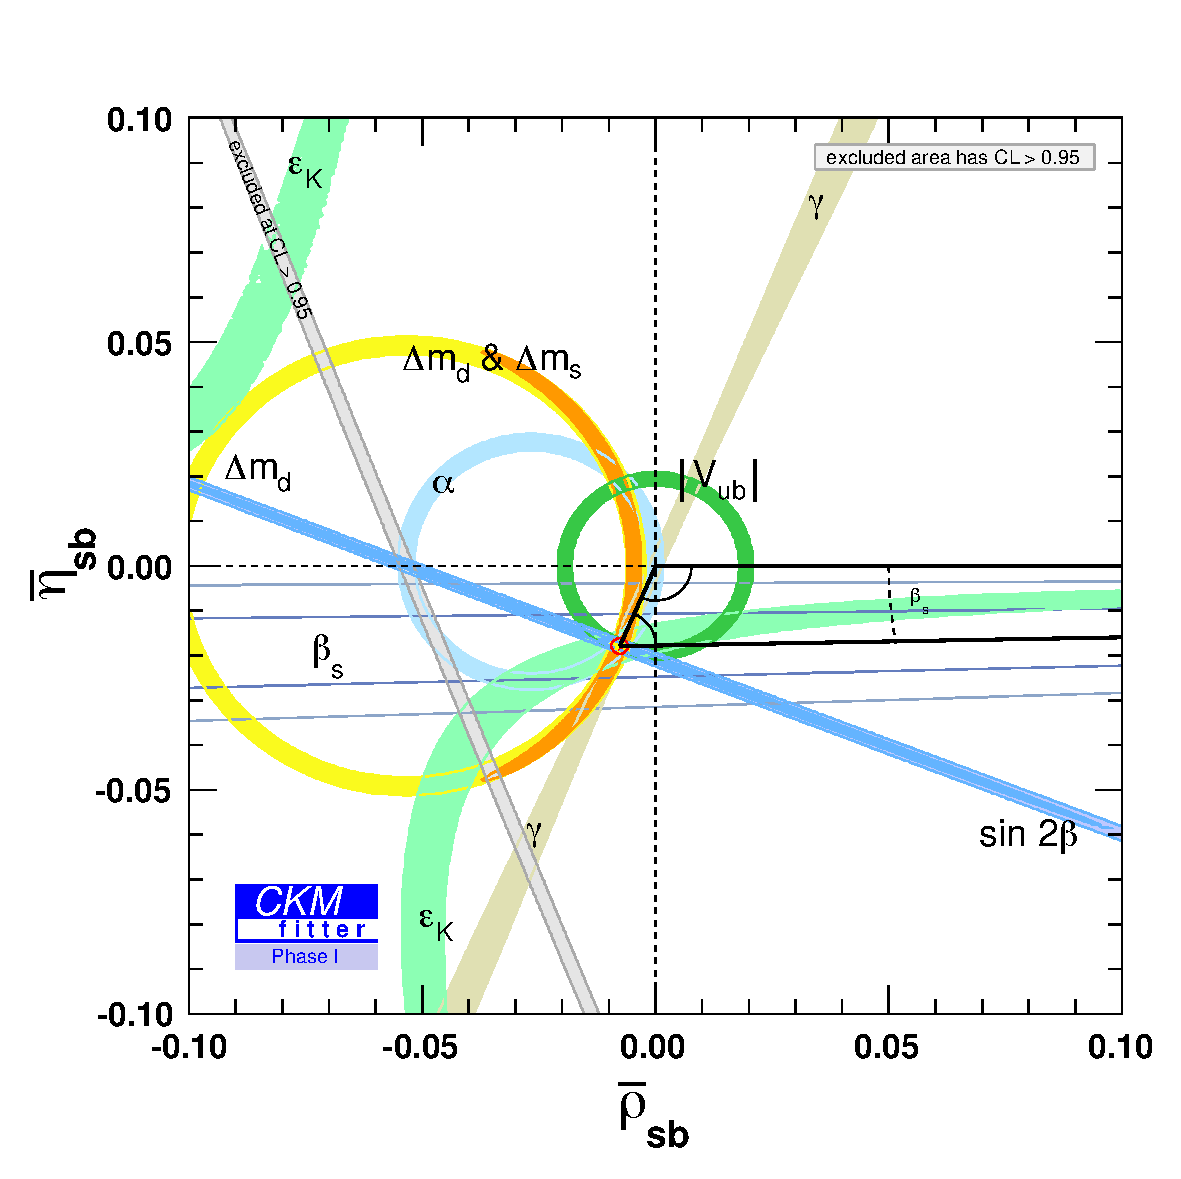
\includegraphics[width=0.45\linewidth]{section2/figures/rhoetaBs_large_Stage1.pdf} 
\includegraphics[width=0.45\linewidth]{section2/figures/rhoetaBs_large_Stage2.pdf} 
\caption{Constraints on the Unitarity Triangle for the $B_s$ meson from the CKMfitter global analysis for phase 1 (left) and phase 2 (right). \td{did we define $\bar \rho_{sb}$ and $\bar \eta_{sb}$ somewhere?}}
\label{fig:CKMfitterglobalBs}
\end{center}
\end{figure}


\begin{figure}
\begin{center}
\centering
\includegraphics[width=0.45\linewidth]{section2/figures/rhoeta_small_global_Stage1.pdf} 
\includegraphics[width=0.45\linewidth]{section2/figures/rhoeta_small_global_Stage2.pdf} 

\includegraphics[width=0.45\linewidth]{section2/figures/rhoeta_small_tree_nogammaimproved_Stage1.pdf} 
\includegraphics[width=0.45\linewidth]{section2/figures/rhoeta_small_tree_nogammaimproved_Stage2.pdf} 

\includegraphics[width=0.45\linewidth]{section2/figures/rhoeta_small_loop_Stage1.pdf} 
\includegraphics[width=0.45\linewidth]{section2/figures/rhoeta_small_loop_Stage2.pdf} 


\caption{Constraints on the Unitarity Triangle for the Unitarity triangle from the CKMfitter global analysis: global fit (top), tree only (center), loop only (bottom),  for phase 1 (left) and phase 2 (right).}
\label{fig:CKMfitterglobalsmall}
\end{center}
\end{figure}


\subsubsection{UTfit results}
The projection of the UT analysis in the HL-LHC era is obtained by performing a global fit using expected values of experimental and theoretical input parameters, as discussed in this Chapter \td{cite more precisely}. In particular, lattice uncertainties in 2025 are taken from table~\ref{table:Proj},  Section~\ref{sec:lattice}. Given this timescale, we use  experimental uncertainties expected at the end of Run 3 for LHCb \td{is this 23 or $50 {\rm fb}^{-1}$, i.e. is this equivalent of Phase 1 of CKMfitter?} and with the full statistics for Belle II. Central values for both theoretical and experimental parameter are taken from a SM point in order to ensure the compatibility of the extrapolated constraints. In Table~\ref{tab:utfit_global_inpout} we summarize the extrapolated uncertainties used in the fit. 

\begin{table}
\caption{Extrapolated input parameter uncertainties used in the UTfit analysis. \td{Phase 1? What about Phase 2?}} 
\label{tab:utfit_global_inpout}
  \begin{center}
	\begin{tabular}{cccccccc}
		\hline \hline
		 Input & Uncer. & Input & Uncer. & Input & Uncer. & Input & Uncer.
		 \\\hline
		 $m_t$ & $0.25$ GeV & $m_b$ & $10$ MeV & $m_c$ & $5$ MeV & $V_{us}$ & $4\times 10^{-4}$
		 \\
		 $|V_{cb}|$ & $4\times 10^{-4}$ & $|V_{ub}|$ & $4\times10^{-5}$ & $|V_{ub}/V_{cb}|$ & $8\times 10^{-4}$ & $\Delta M_d$ & $2\times 10^{-4}$
		 \\
		 $\Delta M_s$ & $6\times 10^{-3}$ & $\sin2\beta$ & $5\times10^{-3}$ & $\alpha$ & $1^\circ$ & $\gamma$ & $1^\circ$
\\
 		 $A_\mathrm{SL}^d$ & $5\times 10^{-4}$ & $A_\mathrm{SL}^s$ & $7\times 10^{-4}$ & $\phi_{B_s}$  & $0.01$ & $B_K$ & $5\times10^{-3}$
		 \\
 		 $F_{B_s}$ & $1\times10^{-3}$ & $F_{B_s}/F_{B_d}$ & $6\times10^{-3}$
 		 & $B_s/B_d$ & $5\times10^{-3}$ & $B_s$ & $7\times10^{-3}$ \\\hline \hline
	\end{tabular} 
\end{center}
\end{table}

The improvement of the UT global analysis can be appreciated in Fig.~\ref{fig:UTfitFut}, where the present and future constraints on the UT plane
are shown next to each other, after zooming on the SM preferred region.

\begin{figure}
\begin{center}
\centering
\includegraphics[width=0.45\linewidth]{section2/figures/utfit_zoom18.pdf} 
\includegraphics[width=0.45\linewidth]{section2/figures/utfit_zoomfut.pdf} 
\caption{Present (left) and future (right) constraints in the $(\bar \rho, \bar \eta)$ plane (UTfit collaboration).}
\label{fig:UTfitFut}
\end{center}
\end{figure}

To be more quantitative, we collect in Table~\ref{tab:utfit_global} the uncertainties of the indirect determination of CKM parameters and angles, obtained from the predictive posterior p.d.f.'s (namely obtained without including the corresponding direct measurements in the fit). These uncertainties are reduced by a factor 3--5,
allowing for an improved test of the SM, as discussed in the next section.

\begin{table}
\caption{Relative uncertainties of UT parameters and angles with current and extrapolated input values for measurements and theoretical parameters (UTfit collaboration).} 
\label{tab:utfit_global}
  \begin{center}
	\begin{tabular}{cccccccc}
		\hline\hline 
		 & $\bar{\rho}$ & $\bar{\eta}$ & $A$ &  $\sin2\beta$ & $\gamma$ & $\alpha$ & $\beta_s$ \\ \hline
		present & 9\% & 3\% & 1.5\% & 4.5\% & 3\% & 2.5\% & 3\% \\ 
		future  & 2\% & 0.7\% & 0.6\% & 0.6\% & 0.5\% & 0.7\% & 0.7\%\\ \hline 	\hline
	\end{tabular} 
\end{center}
\end{table}

\subsection{Future extrapolation of constraints on NP in $\Delta F=2$
  amplitudes}
\label{sec:DF2NP}

% Luca Silvestrini and Marco Ciuchini

The Unitarity Triangle Analysis can be generalized beyond the SM to
obtain a simultaneous determination of CKM parameters and of NP
contributions to $\Delta F=2$ amplitudes \cite{Bona:2007vi}. Assuming
that NP is absent (or negligible) in charged current amplitudes, but
allowing it to be present in FCNC amplitudes, where its virtual
effects compete with loop-level SM amplitudes, we can still use the
measurements of $\vert V_{ud}\vert$, $\vert V_{us}\vert$, $\vert
V_{cb}\vert$, $\vert V_{ub}\vert$, $\gamma$ and $\alpha$ (allowing for
NP contributions in penguins, but barring order-of-magnitude
enhancements of electroweak penguins) to obtain the ``tree-level''
determination of the UT. This allows us
to obtain the SM prediction for $K$, $B_{d}$ and $B_{s}$ mixing
amplitudes; comparing the latter with the experimental results we can
extract $C_{\varepsilon_K} = \varepsilon_K/\varepsilon_K^\mathrm{SM}$
and
\begin{equation}
  \label{eq:cbqphibq}
  C_{B_q} e^{i \phi_{B_q}} = \frac{\langle B_q \lvert H^\mathrm{SM+NP}
    \rvert \bar{B}_q \rangle}{\langle B_q \lvert H^\mathrm{SM}
    \rvert \bar{B}_q \rangle}\,.
\end{equation}
Using semileptonic asymmetries it is possible to break the degeneracy
for $\gamma \leftrightarrow \gamma + 180^\circ$ present in the
tree-level determination of the CKM matrix \cite{Laplace:2002ik},
getting rid of the solution in the third quadrant. We obtain the
results in Tab.~\ref{tab:UTAgen} for the CKM and NP parameters. The
corresponding two-dimensional distributions are shown in
Fig.~\ref{fig:UTAgen}. 

\begin{table}
  \begin{center}
  \caption{Present and future uncertainties on CKM and NP parameters from the generalized UT analysis.
  }   \label{tab:UTAgen}
	\begin{tabular}{cccccccc}
		\hline \hline
		 & $\bar{\rho}$ & $\bar{\eta}$ & $C_{\varepsilon_K}$ &  $C_{B_d}$ & $\phi_{B_d}[^\circ]$ & $C_{B_s}$ & $\phi_{B_s}[^\circ]$ \\ \hline
		present & 0.030 & 0.028 & 0.12 & 0.11 & 1.8 & 0.09 & 0.89 \\ 
		future  & 0.0047 & 0.0040 & 0.036 & 0.030 & 0.28 & 0.026 & 0.29\\ \hline \hline
	\end{tabular} 
\end{center}
\end{table}


\begin{figure}[htb]
\begin{center}
\includegraphics[width=0.45\linewidth]{section2/figures/phibd_cbd-np.pdf}
\includegraphics[width=0.4\linewidth]{section2/figures/cbdvsphibd_fit1.pdf} 
\includegraphics[width=0.45\linewidth]{section2/figures/phibs_cbs-np.pdf}
\includegraphics[width=0.4\linewidth]{section2/figures/cbsvsphibs_fit1.pdf} 
\caption{Present (left) and future (right) constraints on NP contributions to $B_q$-$\bar{B}_q$ mixing.}
\label{fig:UTAgen}
\end{center}
\end{figure}

Combining the results of the generalized UT analysis with the
constraints on CP violation in $D$ mixing from Sec. \td{cite}\textbf{refer to
  $D$ mixing combination}, we can consider the most general $\Delta
F=2$ effective Hamiltonian and bound its coefficients (barring
accidental cancellations).

The most general effective Hamiltonians for $\Delta F=2$ processes
beyond the SM have the following form \cite{Gabbiani:1996hi}:
\begin{eqnarray}
  \label{eq:defheff}
  {\cal H}_{\rm eff}^{K-\bar K}=\sum_{i=1}^{5} C_i\, Q_i^{sd} +
  \sum_{i=1}^{3} \tilde{C}_i\, \tilde{Q}_i^{sd} \\
  {\cal H}_{\rm eff}^{D-\bar D}=\sum_{i=1}^{5} C_i\, Q_i^{uc} +
  \sum_{i=1}^{3} \tilde{C}_i\, \tilde{Q}_i^{uc} \\
  {\cal H}_{\rm eff}^{B_q-\bar B_q}=\sum_{i=1}^{5} C_i\, Q_i^{bq} +
  \sum_{i=1}^{3} \tilde{C}_i\, \tilde{Q}_i^{bq} \nonumber
\end{eqnarray}
where
\begin{eqnarray}
         \label{Qi}
         Q_1^{q_iq_j} & = & \bar q^{\alpha}_{jL} \gamma_\mu
         q^{\alpha}_{iL} \bar q^{\beta}_{jL} \gamma^\mu 
         q^{\beta}_{iL}\; ,
         \nonumber \\
         Q_2^{q_iq_j} & = & \bar q^{\alpha}_{jR}  q^{\alpha}_{iL} \bar
         q^{\beta}_{jR} q^{\beta}_{iL}\; , 
         \nonumber \\
         Q_3^{q_iq_j} & = & \bar q^{\alpha}_{jR}  q^{\beta}_{iL} \bar
         q^{\beta}_{jR} q^{\alpha}_{iL}\; , 
         \\
         Q_4^{q_iq_j} & = & \bar q^{\alpha}_{jR}  q^{\alpha}_{iL} \bar
         q^{\beta}_{jL} q^{\beta}_{iR}\; , 
         \nonumber \\
         Q_5^{q_iq_j} & = & \bar q^{\alpha}_{jR}  q^{\beta}_{iL} \bar
         q^{\beta}_{jL} q^{\alpha}_{iR}\; , 
         \nonumber
\end{eqnarray}
and the operators $\tilde{Q}_{1,2,3}^{q_iq_j}$ are obtained from the
$Q_{1,2,3}^{q_iq_j}$ by the exchange $ L \leftrightarrow R$.  Here
$q_{R,L}=P_{R,L}\,q$, with $P_{R,L}=(1 \pm \gamma_5)/2$, and $\alpha$
and $\beta$ are colour indices.

Following the procedure detailed in ref.~\cite{Bona:2007vi}, we obtain
p.d.f.'s for the Wilson coefficients based on the extrapolated UT and
$D$ mixing analyses. For self-consistency, we compute the coefficients
at a scale $\mu_H$ roughly corresponding to the bound on the NP scale
$\Lambda$ that one can obtain from the analysis (see below). The
allowed regions at $95\%$ probability are reported in Table
\ref{tab:DF2Cbounds}. The regions for $\tilde{C}_i$ are identical to
the ones for the corresponding $C_i$.

In general, the coefficients at the NP scale can be written as
\begin{equation}
  \label{eq:CiLambda}
  C_i(\Lambda) = \frac{F_i L_i}{\Lambda^2}\,,
\end{equation}
where $\Lambda$ is the NP scale corresponding to the new heavy
particles mediating the $\Delta F=2$ transition, $F_i$ is a flavour
coupling and $L_i$ is the overall strength, \textit{e.g.} a loop
factor. For a strongly-interacting NP model with arbitrary flavour
structure one expects $F_i \sim L_i \sim 1$, so with this assumption
we can convert the allowed regions for $C_i$ in the lower bounds on the
NP scale $\Lambda$ reported in Table \ref{tab:DF2Cbounds} and in
Fig. \ref{fig:DF2Lambda}.

\begin{table}[!h]
\begin{center}
\caption{95\% probability ranges for the the Wilson coefficients in Eq.~\ref{eq:defheff} and corresponding bounds on the NP scale. See text for details.}
\label{tab:DF2Cbounds}
\begin{tabular}{@{}cccc}
\hline\hline
Parameter &~~ $95\%$ allowed range~~ &~~ Lower limit on $\Lambda$ (TeV)\\
\hline \hline
$\mathrm{Im} C_K^1$  & $[-3.4,7.0] \cdot 10^{-16}$  &  $37.9\cdot 10^{3}$  \\ 
$\mathrm{Im} C_K^2$  & $[-7.7,3.8] \cdot 10^{-18}$  &  $359.8\cdot 10^{3}$ \\ 
$\mathrm{Im} C_K^3$  & $[-5.2,10.4] \cdot 10^{-17}$  &  $98.2\cdot 10^{3}$ \\ 
$\mathrm{Im} C_K^4$  & $[-8.0,16.0] \cdot 10^{-19}$  &  $789.5\cdot 10^{3}$ \\ 
$\mathrm{Im} C_K^5$  & $[-1.6,3.2] \cdot 10^{-17}$  &  $176.0\cdot 10^{3}$ \\ 
$\mathrm{Im} C_D^1$  & $[-1.4,1.4] \cdot 10^{-15}$  &  $27.1\cdot
10^{3}$ \\
$\mathrm{Im} C_D^2$  & $[-2.2,2.2] \cdot 10^{-16}$  &  $66.8\cdot
10^{3}$  \\
$\mathrm{Im} C_D^3$  & $[-3.3,3.3] \cdot 10^{-15}$  &  $17.4\cdot 10^{3}$   \\
$\mathrm{Im} C_D^4$  & $[-5.5,5.5] \cdot 10^{-17}$  &  $134.5\cdot 10^{3}$ \\ 
$\mathrm{Im} C_D^5$  & $[-6.6,6.5] \cdot 10^{-16}$  &  $39.0\cdot 10^{3}$  \\ 
$|C_{B_d}^1|$  & $< 1.9\cdot 10^{-13}$  &  $2.3\cdot 10^{3}$  \\ 
$|C_{B_d}^2|$  & $< 5.4\cdot 10^{-14}$  &  $4.3\cdot 10^{3}$  \\ 
$|C_{B_d}^3|$  & $< 2.0\cdot 10^{-13}$  &  $2.2\cdot 10^{3}$  \\ 
$|C_{B_d}^4|$  & $< 1.6\cdot 10^{-14}$  &  $7.9\cdot 10^{3}$  \\ 
$|C_{B_d}^5|$  & $< 4.5\cdot 10^{-14}$  &  $4.7\cdot 10^{3}$  \\ 
$\mathrm{Re} C_{B_s}^1$  & $[-4.6,5.9] \cdot 10^{-12}$  &  $411.7$   \\ 
$\mathrm{Re} C_{B_s}^2$  & $[-1.6,1.3] \cdot 10^{-12}$  &  $782.5$   \\ 
$\mathrm{Re} C_{B_s}^3$  & $[-4.7,6.0] \cdot 10^{-12}$  &  $408.2$   \\ 
$\mathrm{Re} C_{B_s}^4$  & $[-3.9,5.0] \cdot 10^{-13}$  &  $1.4\cdot 10^{3}$  \\ 
$\mathrm{Re} C_{B_s}^5$  & $[-1.1,1.4] \cdot 10^{-12}$  &  $842.2$  \\ 
$\mathrm{Im} C_{B_s}^1$  & $[-2.0,2.0] \cdot 10^{-12}$  &  $705.7$  \\ 
$\mathrm{Im} C_{B_s}^2$  & $[-5.5,5.5] \cdot 10^{-13}$  &  $1.3\cdot 10^{3}$  \\ 
$\mathrm{Im} C_{B_s}^3$  & $[-2.1,2.0] \cdot 10^{-12}$  &  $696.7$  \\ 
$\mathrm{Im} C_{B_s}^4$  & $[-1.7,1.7] \cdot 10^{-13}$  &  $2.4\cdot 10^{3}$   \\ 
$\mathrm{Im} C_{B_s}^5$  & $[-4.8,4.8] \cdot 10^{-13}$  &  $1.4\cdot 10^{3}$  \\ 
 \hline\hline
\end{tabular}
\end{center}
\end{table}

\begin{figure}[htb]
\begin{center}
\includegraphics[width=0.6\linewidth]{section2/figures/df2-npscale-cernyb.pdf}
\caption{Present (lighter) and future (darker) constraints on the NP scale from the UTfit NP analysis.}
\label{fig:DF2Lambda}
\end{center}
\end{figure}


\textbf{It would be nice to have a few lines of comparison with bounds
from other sectors like EW or Higgs taken from other chapters of the
YB. Maybe editors can add them during the final editing.}

\end{document}
